\documentclass[12pt, a4paper, openany]{report}

\def\VersionRapport{1.0}

\usepackage[utf8]{inputenc} % un package
\usepackage[T1]{fontenc}      % un second package
\usepackage[francais,english]{babel}  % un troisième package
\usepackage{layout}
\usepackage[top=2.7cm, bottom=2.5cm, left=3.5cm, right=3cm]{geometry}
\usepackage{setspace}

\frenchbsetup{StandardLists=true} % à inclure si on utilise \usepackage[french]{babel}
\usepackage{enumitem}
\usepackage{amssymb}

\usepackage{color}
\usepackage{listings}
\definecolor{dkgreen}{rgb}{0,0.6,0}
\definecolor{gray}{rgb}{0.5,0.5,0.5}
\definecolor{mauve}{rgb}{0.58,0,0.82}
\definecolor{rougecerise}{rgb}{0.73,0.043,0.043}

\lstset{frame=tb,
  language=Java,
  aboveskip=3mm,
  belowskip=3mm,
  showstringspaces=false,
  columns=flexible,
  basicstyle={\small\ttfamily},
  numbers=none,
  numberstyle=\tiny\color{gray},
  keywordstyle=\color{blue},
  commentstyle=\color{dkgreen},
  stringstyle=\color{mauve},
  breaklines=true,
  breakatwhitespace=true,
  tabsize=3
}

\usepackage{multirow} % pour les tableaux
\usepackage[table]{xcolor} % pour les tableaux

\usepackage{graphicx}
\usepackage{caption}
\usepackage{subcaption}
\usepackage {subcaption} 
\usepackage{verbatim}
\usepackage{pifont}
\usepackage{amsmath}
\usepackage{moreverb}
\usepackage{url}
\usepackage{pst-all}
\usepackage{eso-pic,graphicx}
\usepackage{caption} 
\usepackage[colorlinks=true,urlcolor=blue,linkcolor=red]{hyperref}
\usepackage{array}
\usepackage[toc,page]{appendix}
\usepackage[off]{auto-pst-pdf}
\usepackage[upright]{fourier}
\usepackage{hyperref} % pour le sommaire table des matières
\AddThinSpaceBeforeFootnotes % à insérer si on utilise \usepackage[french]{babel}
\FrenchFootnotes % à insérer si on utilise \usepackage[french]{babel}
\usepackage{fancyhdr}
\pagestyle{headings}

\selectlanguage{francais}
\pagenumbering{arabic} 

\renewcommand{\appendixpagename}{Annexes}
\renewcommand{\appendixtocname}{Annexes}

\title{Theme: Performance & Robustesse}
\author{Ali \bsc{Kherbiche}}
\date{2018-2019}



%new
\newcommand{\HRule}{\rule{\linewidth}{0.5mm}}


\begin{document}



\makeatletter
  \begin{titlepage}
  

  \begin{sffamily}
   \begin{center}

    % Upper part of the page. The '~' is needed because \\
    % only works if a paragraph has started.
    
\includegraphics[scale=0.5]{Logo_UT3.jpg}~\\[1.5cm]

    \textsc{\LARGE UFR EEA }\\[2cm]
    
    %\textsc{\Large Rapport Performance et Robustesse}\\[1.5cm]
    
    \textsc{\Large Rapport analyse et performances des systèmes linéaires}\\[1cm]

    % Title
    \HRule \\[0.4cm]
    \textsc{ \huge Asservissement d'un système à trois bacs d'eau\\[0.4cm] }

    \HRule \\[2cm]
    
\includegraphics[width=3cm,height=3cm,keepaspectratio] {cropped-Logo-master-EEA.jpg}
    \\[2cm]

    % Author and supervisor
    \begin{minipage}{0.4\textwidth}
      \begin{flushleft} \large
         \textsc{Kherbiche Ali}\\
         \textsc{Halimi Amine}\\
        \emph {Promotion:} \\
         \textsc{2018-2019}\\
      \end{flushleft}
    \end{minipage}
    \begin{minipage}{0.4\textwidth}
      \begin{flushright} \large
        \emph{Encadreur et Responsable de la Formation M1 ISTR-RODECO :}  \textsc{M. Frédéric GOUAISBAUT}\\
        %\emph{Responsable de la Formation:} \textsc{M. BIDON}
      \end{flushright}
    \end{minipage} 

    \vfill

    % Bottom of the page
    \emph{\large Novembre 2018}

  \end{center}
  \end{sffamily}      
          
  \end{titlepage}
  
\makeatother



% *********************** Remerciements *****************
\chapter*{Remerciements}
 \addcontentsline{toc}{chapter}{Remerciements}
  
  \paragraph{}
   Nous tenons à remercier notre encadreur et professeur de cours, M.Frédéric GOUAISBAUT pour nous avoir guidé tout au long des deux séances de travaux pratiques, nous tenons aussi à lui reconnaitre le temps qu'il nous a consacré car il nous a accompagnés tout au long de cette expérience professionnelle avec beaucoup de patience et de pédagogie. \\ 
   
  \paragraph{}
   On pense ici à notre professeur M.Sylvain DUROLA, On le remercie d’avoir été toujours présent durant toutes les séances de travaux dirigés, on le remercie encore de nous avoir donné beaucoup de connaissances techniques et des idées sur le monde du travail.\\
 
  \paragraph{} 
   Enfin nous voudrions adresser ici nos remerciements spéciaux à toute l’équipe pédagogique d’automatique de l'université de Toulouse III qui nous a donné l’occasion de faire nos TP dans d'excellentes conditions.   \\

  \paragraph{}  
  On a trouvé ce bureau d’étude  très intéressant et enrichissant, puisqu’il s’agissait pour nous d’un domaine qu'on aurait souhaité exercer dans le futur. \\
   
%*********************** somaire **************
\tableofcontents
%*********************** listes des figures **************
\listoffigures
%*********************** listes des tableaux **************
%\listoftables



%*********************** INTRODUCTION **************
\chapter*{Introduction}
 \addcontentsline{toc}{chapter}{Introduction}
 
 \section*{Performance}
 
 \paragraph{Définition:} Le modèle de performance de Gilbert (1980) décrit la performance dans une relation ternaire entre les objectifs visés (cibles, estimations, projections), les moyens pour les réaliser (les ressources humaines, matérielles, financières ou informationnelles) et les résultats obtenus (biens, produits, services, etc.). Cette définition de la performance s'applique à tout système ordonné (individu, organisation, système, etc.) qui produit des résultats à partir de ressources de base.\cite{ref3}
 
 \paragraph{Définition en automatique:} Plusieurs paramètres caractérisent les performances d'un asservissement :

 \begin{itemize} [label=\ding{70},font=\small \color{black}]
  	\item La rapidité définit par la vitesse à laquelle une valeur stable en sortie est atteinte. C'est le temps de réponse. 
    \item La stabilité. Pour une entrée constante, un système est stable si la sortie tend vers une valeur finie. Si elle oscille ou diverge, l'asservissement est instable. 
    \item Le dépassement de la consigne, souvent exprimé en pourcentage d'erreur. Même lorsqu'un système est stable, il arrive que la sortie dépasse la consigne avant de se stabiliser, ce qui n'est pas nécessairement une anomalie.
   \item La précision, c’est-à-dire la capacité de l'asservissement à atteindre la consigne avec précision le plus rapidement possible.\cite{ref4}
  \end{itemize}
 
 \section*{Robustesse}
 
 \paragraph{Définition:} Force, vigueur en parlant d'une personne. Solidité, en parlant d'une chose.\cite{ref6}
 
 \paragraph{Définition en automatique:}  En ingénierie, la robustesse d'un système se définit comme la « stabilité de sa performance ». Les systèmes performants robustes, qui restent performants malgré des conditions externes présentant de larges variations d'amplitude (exemple : variation de température, d'adhérence au sol, dispersion d'usinage...)
 
 \begin{itemize} [label=\ding{70},font=\small \color{black}]
  	\item Réseau Internet (performance = croissance rapide des interconnexions machines - robustesse = communication inter-machines maintenue en cas d'attaque nucléaire). 
    \item Train TGV (performance = train rapide - robustesse = haute stabilité de la trajectoire en cas de déraillement). 
    \item Avion Airbus A320 (performance = communité de la cabine de pilotage 318-321, commandes électriques de vol - robustesse = vol possible avec un réacteur en panne).
    \item Fusée Ariane 4.\cite{ref5}
  \end{itemize}
 
 
 
 \section*{Objectif}
  Le but de cette manipulation est d'illustrer la commande robuste d'un système non linéaire linéarisé autour d'un point de fonctionnement et de mettre en oeuvre les techniques d'analyse et de synthèse de lois de commande robuste comme le loop-shapping.\\
                                                      



%*********************** Problématique **************
\chapter*{Problématique}
 \addcontentsline{toc}{chapter}{Problématique}
 
 \paragraph{}
Le système représenté sur ci-dessous est composé de trois bacs cylindriques en plexiglas de section $S$. Ces trois bacs sont disposés en série (de gauche à droite, on trouve lesbacs 1, 3 et 2) et sont reliés par des tuyaux d’écoulement de section $S_{n}$. Le dernier bac (2) se vide par un cylindre – également de section $S_{n}$ – dans un réservoir situé sous les bacs. Deux pompes de débit $Q_{1} (t)$ \hspace{1mm}et \hspace{1mm}$Q_{2} (t)$ permettent de remplir respectivement les bacs 1 et 2 avec l’eau récupérée dans le réservoir, le systéme fonctionnant en circuit fermé. Lors de cette manipulation, nous allons nous intéresser à la régulation de niveau d’eau dans les bacs. Les niveaux, notés $H_{1} (t)$, $H_{3} (t)$\hspace{1mm} et \hspace{1mm}$ H_{2} (t)$ ne peuvent excéder la valeur de $0.6 m$. Les valeurs données par le constructeur sont : $S = 0.0154m^{2}$\hspace{1mm} et\hspace{1mm} $S_{n} = 5.10^{-5} m^{2} $. Une armoire de commande, reliée au procédé, permet de commander (en tension) les deux pompes et de mesurer (en tension) les trois hauteurs d’eau dans les bacs par l’intermédiaire de capteurs de niveau; ces capteurs sont basés sur la mesure de la pression dans les bacs. 
 
 \begin{center}
   %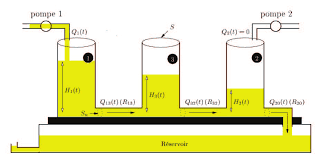
\includegraphics[width=12cm]{index.png}
   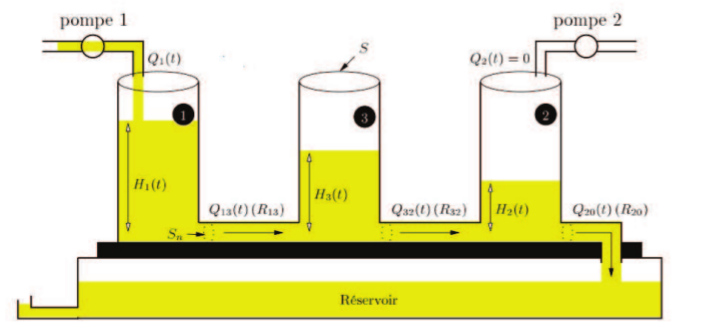
\includegraphics[width=13cm]{rebout.png}
   \captionof{figure}{\textit{Procédé trois bacs \cite{ref1}}}
   \label{fig1}
 \end{center}   
  
 \paragraph{}
L’armoire de commande est à son tour pilotée par une carte DSPACE (type DS1102)
équipée de Convertisseurs Analogique-Numérique et Numérique-Analogique, ainsi que de
processeurs DSP \textit{(Digital Signal Processing)} ; cette carte est interfacée avec SIMULINK.
D’autre part, nous souhaitons travailler sur des faibles variations autour du point
d’équilibre \hspace{1mm}$H_{0}$\hspace{1mm} ; nous noterons par des lettres minuscules les variations des signaux autour
de ce point de telle sorte que :

\[\left \{
   \begin{array}{r c l}
      Q_{1}(t)  & = & q_{1}(t)+Q_{10} \\
      H_{1}(t)  & = & h_{1}(t)+H_{10} \\
      H_{2}(t)  & = & h_{2}(t)+H_{20} \\
      H_{3}(t)  & = & h_{3}(t)+H_{30} \\
   \end{array}
   \right .\]
 
 \paragraph{}
 La fonction de transfert entre le débit d’entrée \hspace{1mm}$q_{e}(t)$\hspace{1mm} et la sortie \hspace{1mm}$h_{1}(t)$ \hspace{1mm}est alors donnée par :\\[0.75mm]
 
 \begin{Large}
 \begin{center}
 $\frac{q_{e}(t)}{h_{1}(t)}  =  \frac{16p+20}{p^{3}+7p^{2}+12.75p+6.75} $
  \end{center}
 \end{Large}
 
 \paragraph{}   
 Notre système est soumis à des perturbations exogènes suivants:
        
  \begin{enumerate}
      \item Un débit de fuite constante au niveau du bac numéro 1.
      \item Un bruit de mesure sur le capteur permettant la mesure de $h_{1}(t)$.
  \end{enumerate} 
 
 \paragraph{}
 Nous désirons alors effectuer un asservissement permettant d’assurer les spécifications
suivantes :

\begin{enumerate} [label=(\alph*)]
 \item La stabilité du système en boucle fermée,
 \item Une erreur de position nulle,
 \item Une erreur de vitesse limitée à 1 i.e. lorsque l’entrée de consigne est une rampe de
pente 1. 
 \item Une convergence vers la consigne en moins de 3 sec, sans oscillation, ni dépassement,
 \item Un rejet de la perturbation de fuite,
 \item Un rejet du bruit de mesure au delà de\hspace{1mm} $100Hz$ \hspace{1mm}d’au moins\hspace{1mm} $60dB$ \hspace{1mm}par décade.

\end{enumerate} 

%*********************** Performance et Robustesse **************
\chapter{Analyse d'une commande proportionnelle intégrale}

%\chaptermark{Commande proportionnelle intégrale}

 \section{Le schéma bloc du systéme bouclé} 

\paragraph{}
	Après l'ajout du correcteur PI $K(p)= k \frac {1+\tau_{i}p}{\tau_{i}p}$ à notre système, voici à quoi ressemble le       shéma bloc de l'asservissement:
% captures d’écrans 
  \begin{center}
    %
\includegraphics[scale=0.5]{Logo_UT3.jpg}
    \captionof{figure}{\textit{Schéma bloc de l'asservissement}}
    \label{fig2}
  \end{center}    
 
 \paragraph{}
	On voit clairement que le signal du débit de fuite $W_{u}(p)$ du bac numéro 1 est relié au signal de commande $U(p)$ et le signal du bruit de mesure $b(p)$ et relié au signal de sortie $h_{1}(p)$.    
	
 \section{La validité de L'hypothèse} 
  
 \paragraph{}       
	Vu que l'eau est un liquide incompréssible, notre supposition du débit de fuite constant tient la route.
	
 \section{Le diagramme asymptotique de $K(p)= k \frac {1+\tau_{i}p}{\tau_{i}p}$} 
 
 % captures d’écrans 
  \begin{center}
    %
\includegraphics[scale=0.5]{Logo_UT3.jpg}
    \captionof{figure}{\textit{Diagramme de Bode (gain et phase) de $K(jw)$ }}
    \label{fig3}
  \end{center}

  \textbf{Nota:} \hspace{2mm} Le correcteur a une allure d'un filtre passe bas.

 \section{Les spécifications satisfaites}
 
  \begin{itemize} [label=\ding{70},font=\small \color{black}]
  	\item Sans connaître les valeurs numérique du gain $k$ ou celle de la constante de temps $\tau_{i}$ utilisées dans le correcteur $K(p)$, on pourra déjà satisfaire la spécification $(b)$ car un integrateur $\frac{1}{p}$ ce que contient notre correcteur élimine l'erreur de position.
  \end{itemize}
 
 \section{Détermination de la contrainte sur le gabarit de $\xi_{p}$ \hspace{1mm} et \hspace{1mm} $\xi_{v} $ pour $S(p)$}  
 
  \subsection{Construction du gabarit de l'erreur de position}
  
   On dispose de la loi suivante: \hspace{5mm} $\xi_{p}=\underset{p\longrightarrow 0}{lim}  p\xi(p)$\\[0.75cm]
   On sait que: \hspace{5mm} $\xi(p)=S(p)R(p)$\\[0.75cm]
   Avec la consigne qui est égale à: \hspace{5mm} $R(p)=\frac{1}{p}$\\[0.75cm]
   Donc: \hspace{5mm} $\xi_{p}=\underset{p\longrightarrow 0}{lim} S(p)=S(0)$\\[0.75cm]
   Si on choisit la fonction de pondération $W_{1}(p)=\frac{\alpha}{p}$ tel que $|W_{1}(p)S(p)|<1$, alors $|S(p)|<\alpha p$, $\alpha \in R^{*}$ \\[0.75cm]
   On obtient au final: \hspace{5mm} $||S(jw)||_{H\infty}<\alpha jw$, $\alpha \in R^{*}$. Pour valider le choix il suffit de calculer $S(p)$ quand $p\rightarrow0$ qui est égal à $0$, donc $\forall w \in R \hspace{2mm} \xi_{p}=0$ 
   
   \begin{center}
    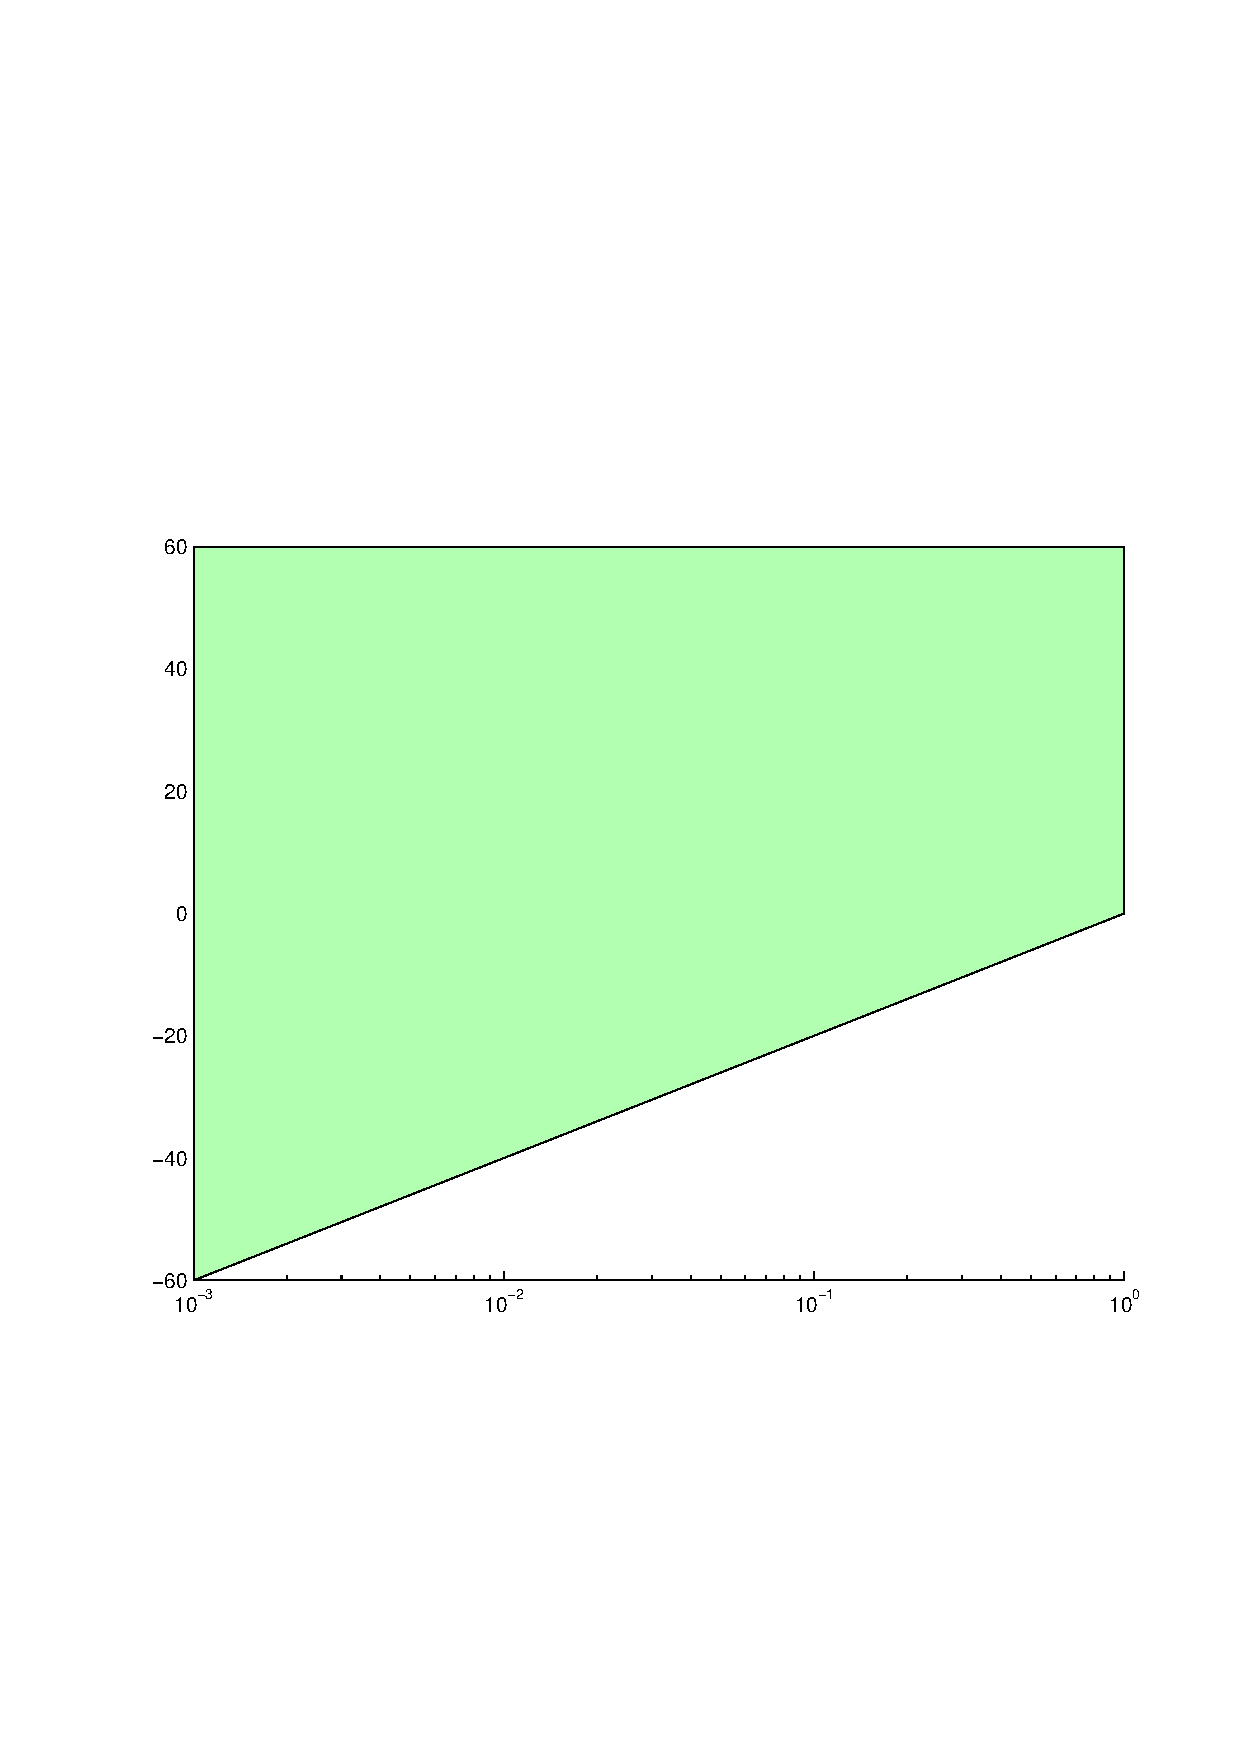
\includegraphics[scale=0.5]{gabarit1.pdf}
    \captionof{figure}{\textit{Diagramme illustrant le gabarit de l'erreur de position}}
    \label{fig4}
  \end{center}

\paragraph{}
Dans notre cas $\alpha$\hspace {1mm}équivaut à \hspace{1mm} $1$.   
   
  \subsection{Contruction du gabarit de l'erreur de vitesse}
  
  Cette fois pour calculer l'erreur de vitesse $\xi_{v}$ le signal de consigne équivaut à $R(p)=\frac{1}{p^{2}}$\\[0.75cm]
  Donc: \hspace{5mm} $\xi_{v}=\underset{p\longrightarrow 0}{lim}\frac{S(p)}{p}$\\[0.75cm]
  Si on choisit la fonction de pondération $W_{2}(p)=\frac{\beta}{p}$ tel que $|W_{2}(p)S(p)|<1$, alors $|S(p)|<\beta p$, $\beta \in ]0, 1]$\\[0.75cm]
  On obtient au final: \hspace{5mm} $||S(jw)||_{H\infty}<\beta jw$, $\beta \in ]0, 1]$. Pour valider le choix il suffit de calculer $S(p)$ quand $p\rightarrow0$ qui est égal à $\beta$, donc $\forall w \in R \hspace{2mm} \xi_{v}=\beta$ 
  
  \begin{center}
    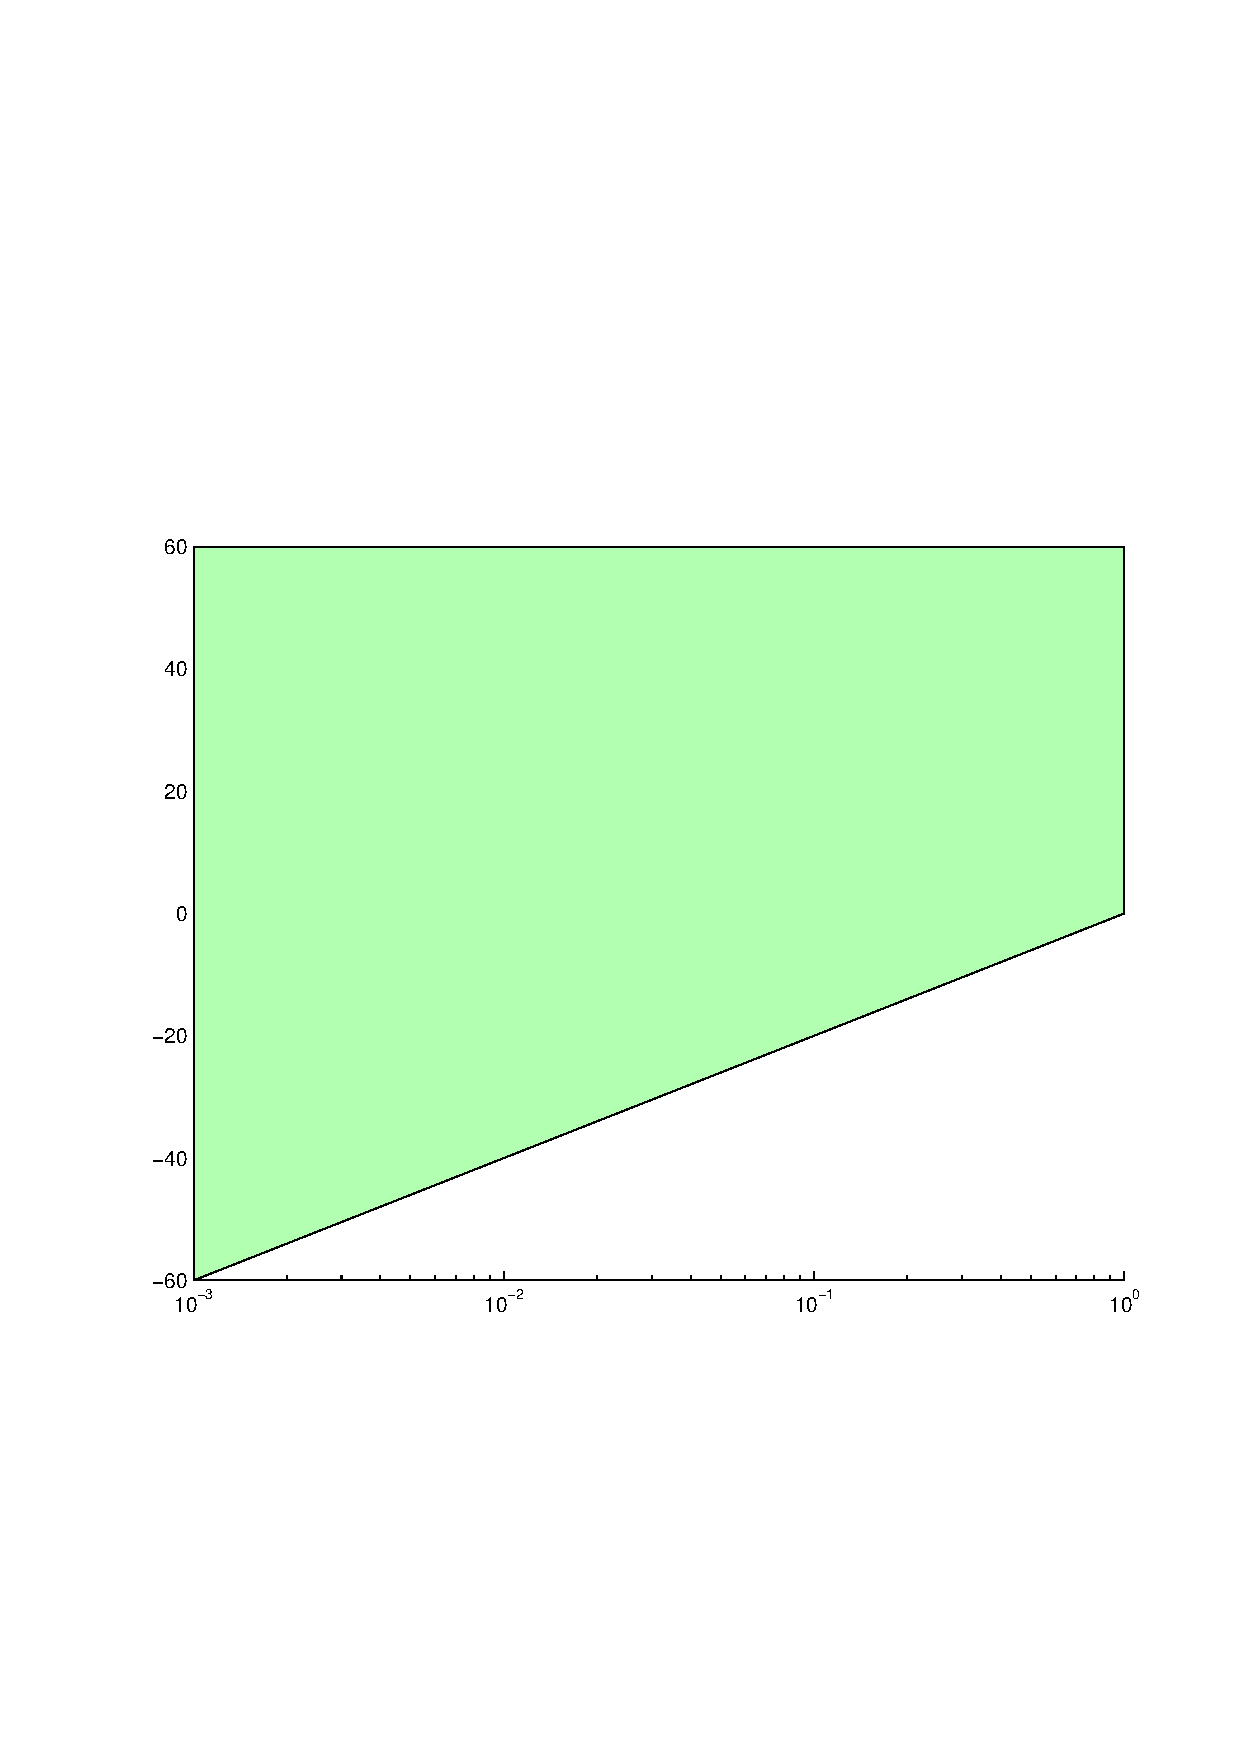
\includegraphics[scale=0.5]{gabarit1.pdf}
    \captionof{figure}{\textit{Diagramme illustrant le gabarit de l'erreur de vitesse}}
    \label{fig5}
  \end{center}
  
 \textbf{Nota:} \hspace{2mm} Les deux gabarits vu précédemment sont soit colinéaires soit l'un est comporté ou et inclut dans l'autre. Dans notre cas $\alpha = \beta = 1$,\hspace {1mm}ainsi $W_{1}(p)=W_{2}(p) $.  \\
 

 \section{La bande passante de $S(p)$}
 
 \paragraph{}
 On dispose de la relation de la bande passante sur $T(jw)$: $|T(jw)|_{dB}-|T(0)|_{dB}>3dB,\hspace{1mm} \forall w\in[0, w_{c}]$, $w_{c}$: pulsation de coupure, on trouvera sa valeur plus tard dans le rapport.\\
 Après développement on obtient: $\frac{|T(jw)|}{|T(0)|}>\frac{1}{\sqrt{2}} \Rightarrow |T(jw)|>\frac{1}{\sqrt{2}}, w\in[0, w_{c}]$ qui est la condition nécéssaire qu'il faut satisfaire afin de créer le gabarit équivalent à la spécification sur la vitesse de convergence.\\
 
 \paragraph{}
 Si on choisit la suivante condition sur $S(jw)$: $|S(jw)|<1-\frac{1}{\sqrt{2}}$ \hspace{1mm} c'est à dire $||S(jw)||_{H\infty}<1-\frac{1}{\sqrt{2}} \hspace{1mm} où \hspace{1mm} w\in[0, w_{c}]$ \\
 $\Rightarrow$ \hspace{3mm} $\frac{1}{\sqrt{2}}<1-|S(jw)|.........(1)$\\
 
 \paragraph{}
 Or on sait que: $|T(jw)|+|S(jw)|\geqslant1$\\
 Ainsi: $1-|S(jw)|\leqslant|T(jw)|.........(2)$\\
 
 \paragraph{}
 De $(1)$ et $(2)$ on obtient: \hspace{5mm} $\frac{1}{\sqrt{2}}<1-|S(jw)|\leqslant|T(jw)|$\\
 Il ne reste qu'à dire que pour \hspace{1mm} $\forall w\in[0, w_{c}],$ \hspace{2mm} $\frac{1}{\sqrt{2}}<|T(jw)|$\\
 
 \paragraph{}
 Au final la fonction de pondération $W_{3}(jw)=\frac{\sqrt{2}}{\sqrt{2}-1}$ \hspace{1mm} s'obtient en validant la condition $|W_{3}(jw)S(jw)|<1.$\hspace{1mm}De cette manière la condition sur $T(jw)$ est respectée, maintenant voyons ce que va donner l'interprétation graphique du gabarit.\\
 
 \section{Construction du gabarit de la vitesse de convergence pour $S(p)$} 
 
  \begin{center}
    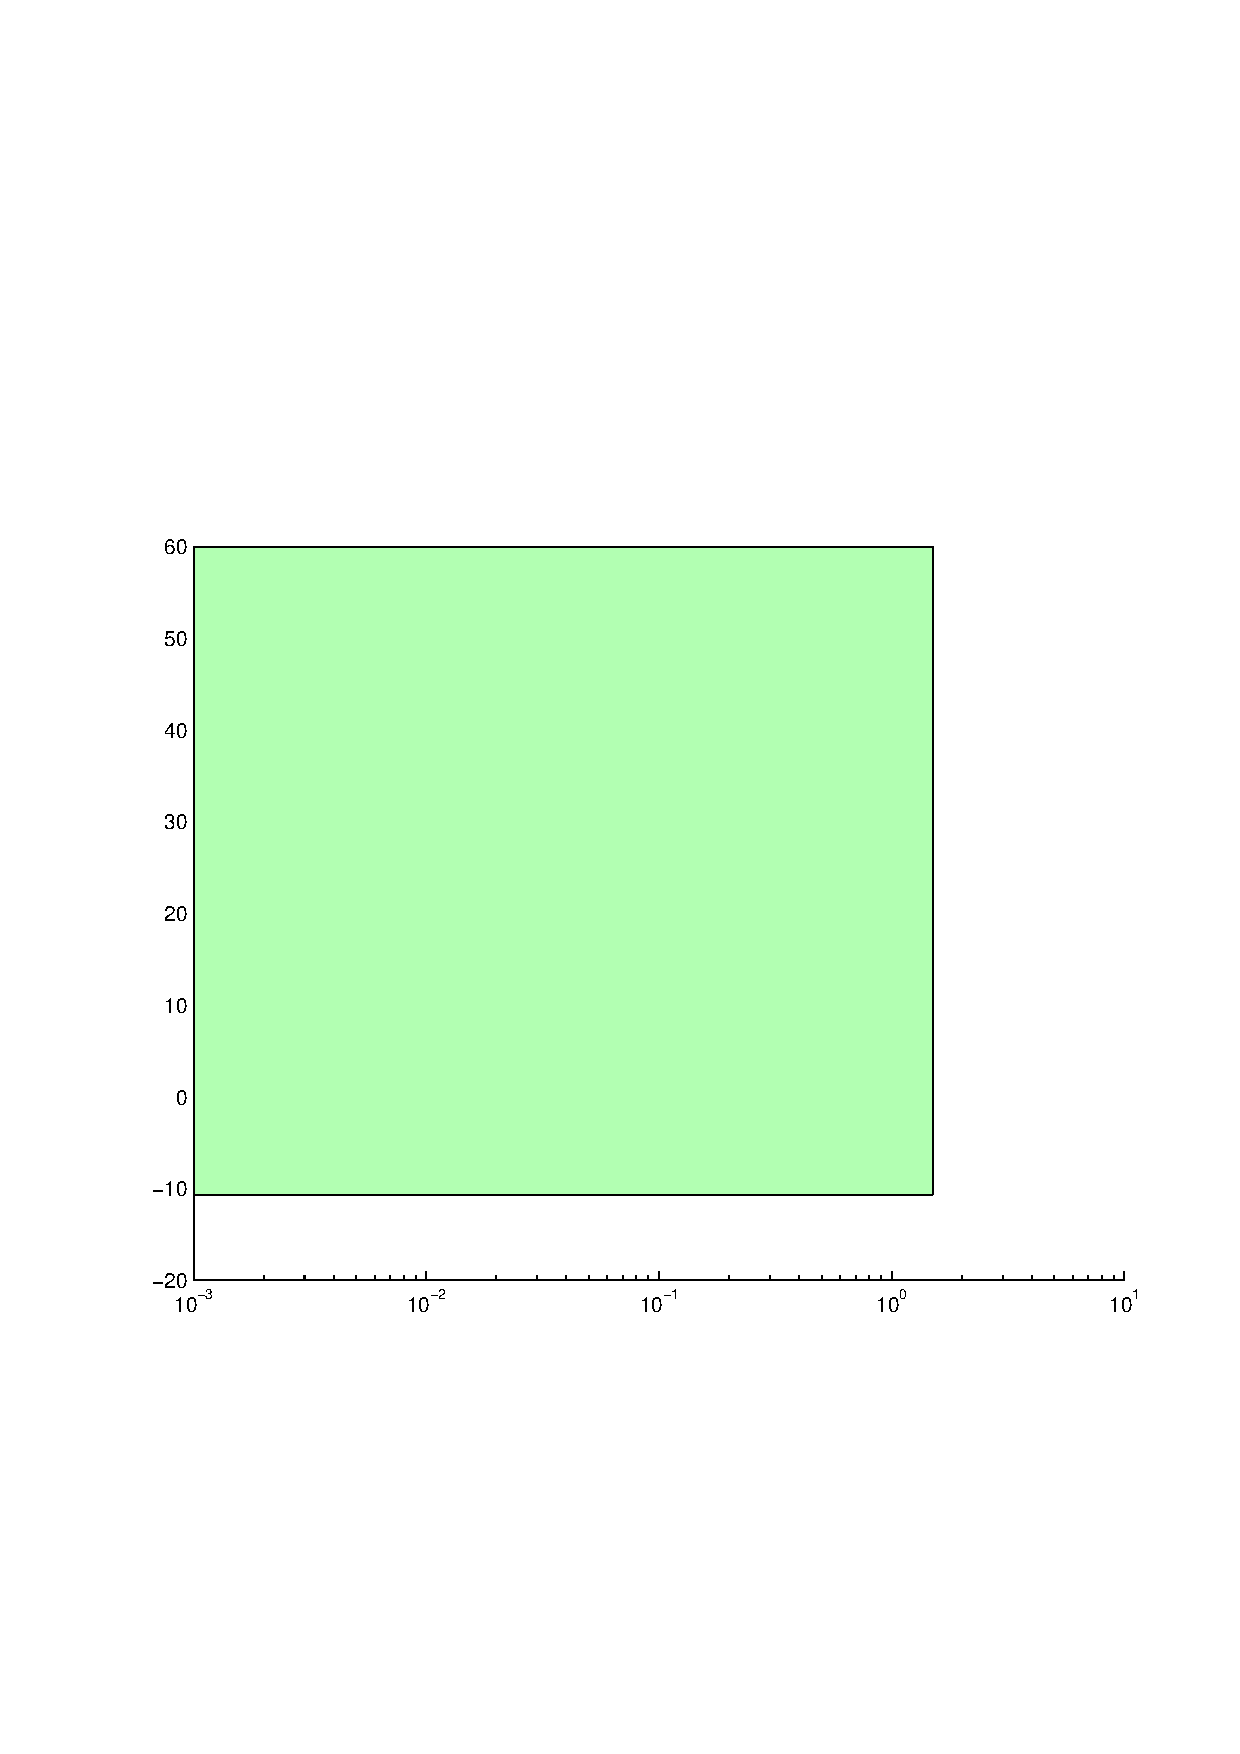
\includegraphics[scale=0.5]{gabarit2.pdf}
    \captionof{figure}{\textit{Diagramme illustrant le gabarit de la vitesse de convergence pour $S(p)$}}
    \label{fig6}
  \end{center}
  
  \paragraph{}
  Du graphe on constate que $|S(jw)|_{dB} < 20log(1-\frac{1}{\sqrt{2}}) = -10.66dB, \forall w\in[0, w_{c}]$. 
  
 \section{Construction du gabarit de la convergance sans oscillations pour $S(p)$} 
  
  \paragraph{}
  Afin de satisfaire cette spécification du cahier des charges nous choisissons de démarrer par la définition de la marge de module $M_{m} $ qui est inversement propertionnelle à la norme H infinie de la fonction de sensiblité $S(p) $, on trouve: $M_{m}=\frac{1}{||S(jw)||_{H\infty}} $ 
 
  \paragraph{}
  On sait que si $ M_{m} > 1 $ alors l'asservissement n'aura ni oscillations ni dépassements. Essayons de développer cette idée: \\
  $M_{m}=\frac{1}{||S(jw)||_{H\infty}} > 1, $ d'ou l'on obtient: \hspace{1mm} $||S(jw)||_{H\infty}<1$ \\
  Si on prend la fonction de pondération suivante: \hspace{1mm} $W_{4}(jw)=1, $ donc la relation: \hspace{1mm} $|S(jw)W_{4}(jw)|<1 $ \hspace{1mm} est vérifiée. Graphiquement on aura le gabarit suivant:\\ 
  
  \begin{center}
    %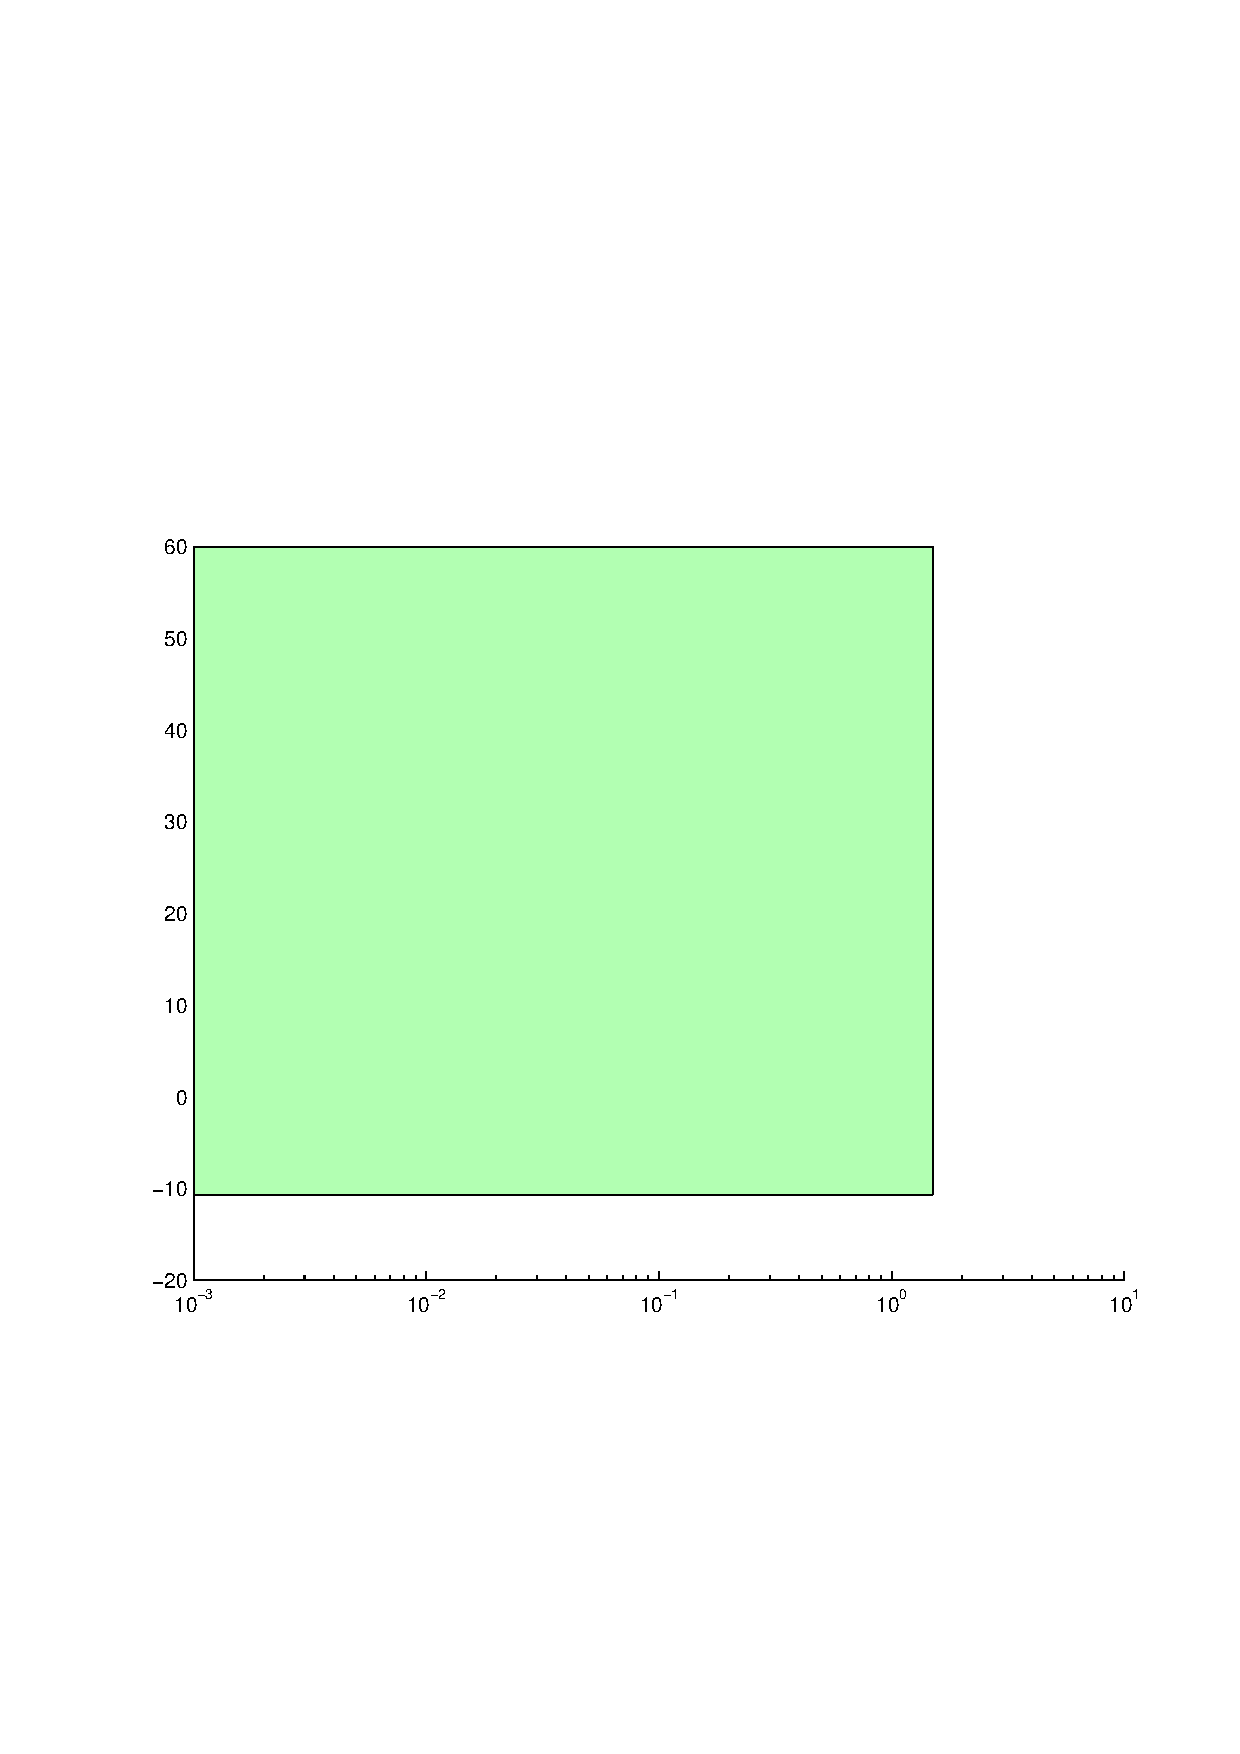
\includegraphics[scale=0.5]{gabarit2.pdf}
    \captionof{figure}{\textit{Diagramme illustrant le gabarit de la convergence sans oscillations pour $S(p)$}}
    \label{fig7}
  \end{center}  
  
  \textbf{Conséquence importante:} \hspace{2mm} On constate que le gabarit choisit ne repsecte pas la limitation liée à l'integrale de Bode car il ne permet pas à la courbe de $S(jw) $ de franchir la partie positive du plan, dans ce cas la réponse temporelle aura forcemment des dépassement ou/et des oscillations ce que le cahier des charges nous permet pas de faire.\\
  
  \paragraph{}
  Disons que notre système est du second ordre ou contient deux modes dominants, sa fonction  de transfert est de la sorte:\hspace{2mm} $ H(p)=\frac{K}{ \frac{p^{2}}{{w_{n}^{2}}} + \frac{2\zeta}{w_{n}} + 1 }$.\hspace{1mm} Afin d'obtenir un système sans oscillations/dépassements, on choisit un coefficient d'ammortissement $\zeta>0.7$, valeur nécéssaire pour éviter les oscillations/dépassements.
  
  \begin{center}
    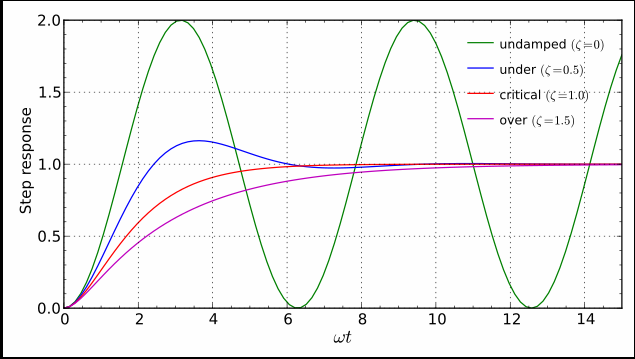
\includegraphics[scale=0.5]{zetaa.png}
    %\includesvg{zeta}
    \captionof{figure}{\textit{Fonctions de transfert du second ordre \cite{ref2}}}
    \label{fig8}
  \end{center}
  
  %BIb:https://he.wikipedia.org/wiki/%D7%A7%D7%95%D7%91%D7%A5:Second_order_transfer_function.svg
  
  Prenons $\zeta=0.91$\hspace{1mm} et calculons la valeur du dépassement $D $\hspace{1mm}:\\
  On sait que:\hspace{1mm}$D_{k}=100e^{\frac{-k \zeta \pi}{\sqrt{1-\zeta^{2}}}} $,\hspace{1mm} $k=1$ dans notre cas.\\
  Après avoir remplacé la valeur de $\zeta$ dans la formule précédente et calculé D puis $D$ en $dB, $ \hspace{1mm} il ne reste qu'à affecter $D_{dB}$\hspace{1mm} à  \hspace{1mm}$W_{4}(jw)$. \hspace{1mm} De cette manière on a construit le bon gabarit.\\
  
  \begin{center}
    %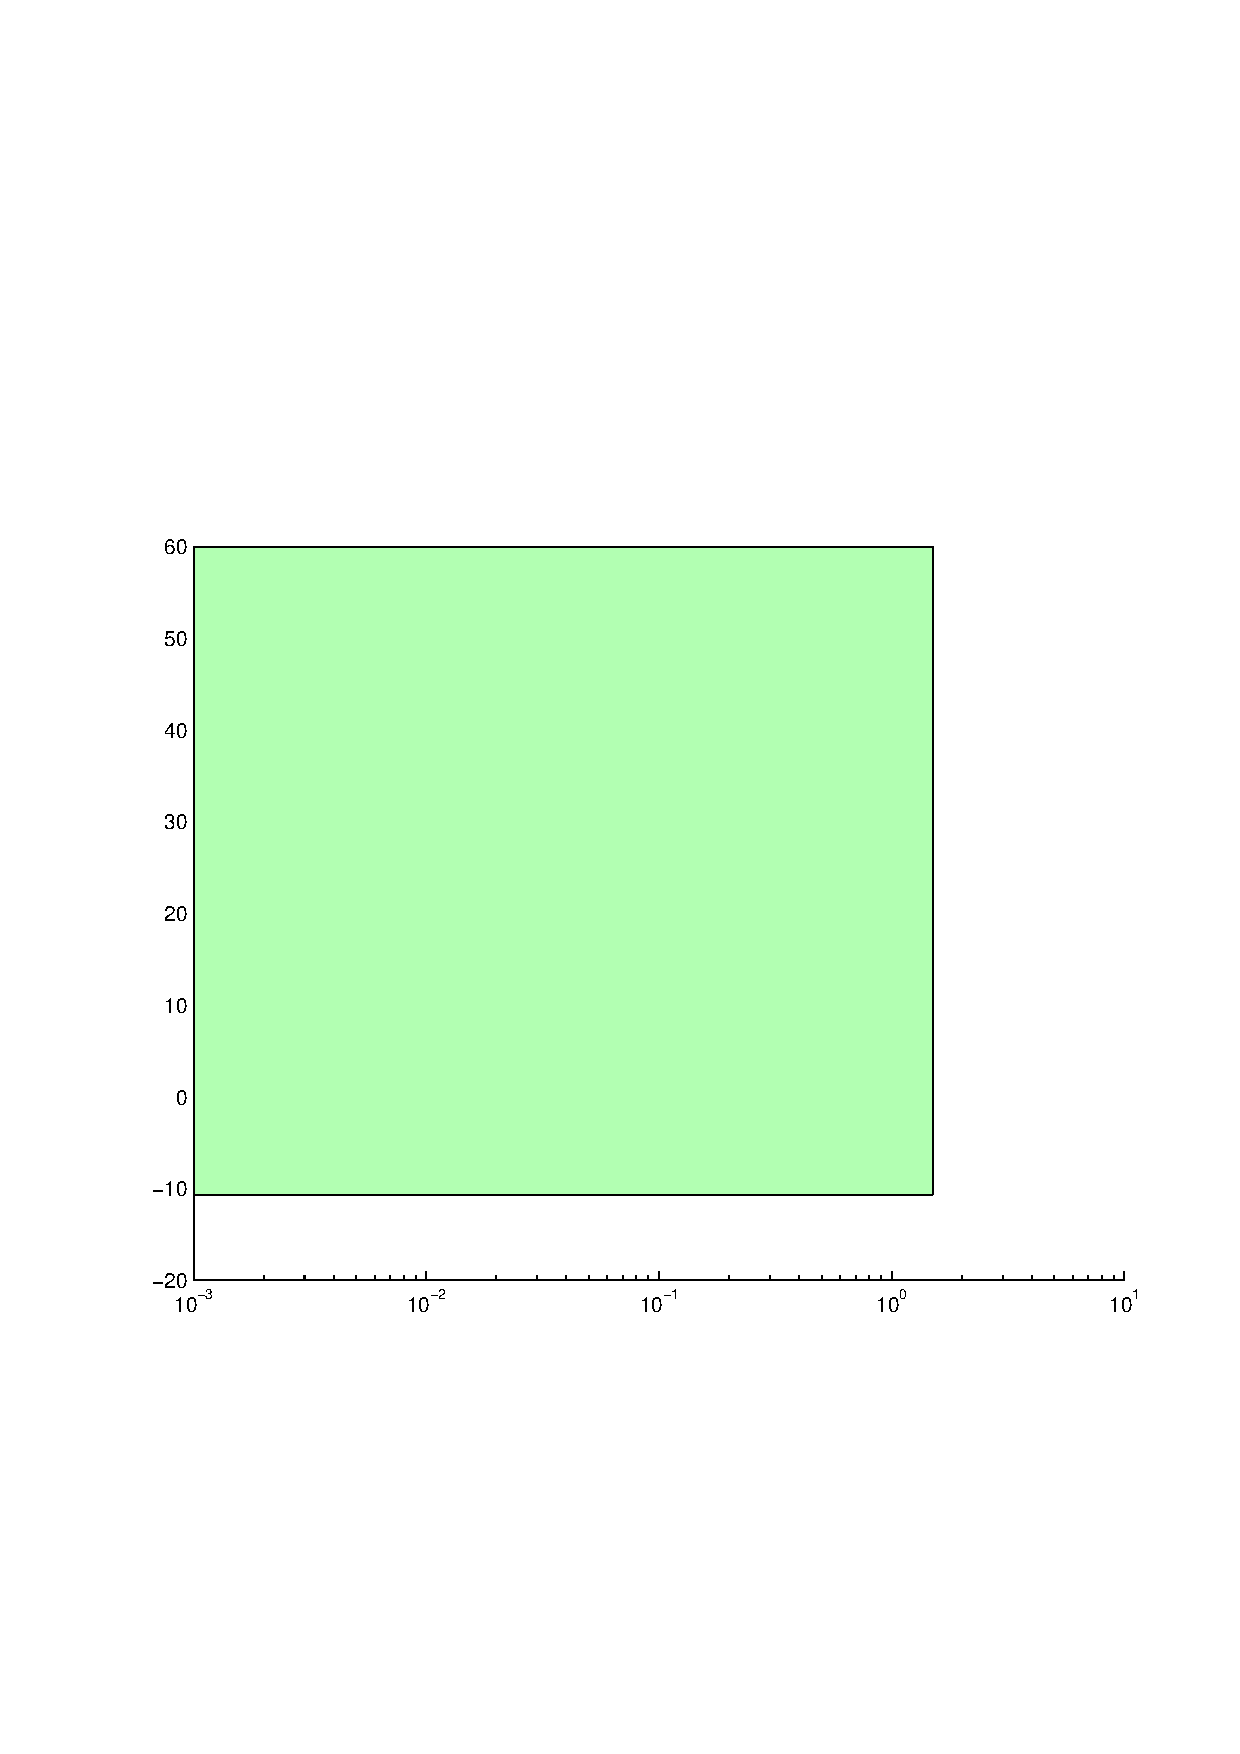
\includegraphics[scale=0.5]{gabarit2.pdf}
    \captionof{figure}{\textit{Diagramme illustrant le gabarit de la convergence sans oscillations pour $S(p)$}}
    \label{fig9}
  \end{center}  


 \section{Construction du gabarit du rejet du bruit de mesure pour $S(p)$}
 
 \paragraph{}
 On doit déterminer un filtre $W_{5}(jw) $\hspace{1mm} de telle sorte que $||W_{5}(jw)T(jw)||_{H\infty} < 1$.\\
 
  \textbf{Supposition:} \hspace{1mm} Puisqu'en général $b(p)$ \hspace{1mm} est un phénomène haute fréquence, alors il faut que $|T(jw)|$ \hspace{1mm} soit petit pour des pulsation assez grandes. Par conséquent $|S(jw)| \simeq 1$ \hspace{1mm} pour des pulsations assez grandes.\\
  
  Afin de respecter notre cahier des charges on pose $|T(jw)|_{dB} \leqslant |\frac{1}{W_{5}(jw)}|_{dB} = -60 dB, \forall w > 200 \pi. $\\   
  D'autres part: \hspace{1mm} $|T(jw)| \leqslant 0.001, $ \hspace{1mm} aussi: \hspace{1mm} $|T(jw)| = |1-S(jw)|, $\hspace{1mm} donc: \hspace{1mm} $1-S(jw) \leqslant 0.001 $  \hspace{1mm} d'ou: \hspace{1mm} $|S(jw)| \geqslant 0.999$ \hspace{1mm} et donc: $|\frac{1}{W_{5}(jw)}|=0.999, \forall w > 200 \pi.$ \\

\paragraph{}
 N'oublions pas que: $S(jw) = 1-T(jw)$ \hspace{1mm} $\Rightarrow$ $|S(jw)|=|1-T(jw)| < 1+|T(jw)|=1.001, \forall w > 200  \pi .$\\  
 Pour conclure: $\forall w > 200 \pi, $ \hspace{1mm} $ 0.999 \leqslant |S(jw)| < 1.001$ \hspace{1mm} ainsi notre supposition est vérifiée.
 
 \paragraph{}
 Voici l'interprétation graphique de ce qu'on vient de voir:\\

\begin{center}
    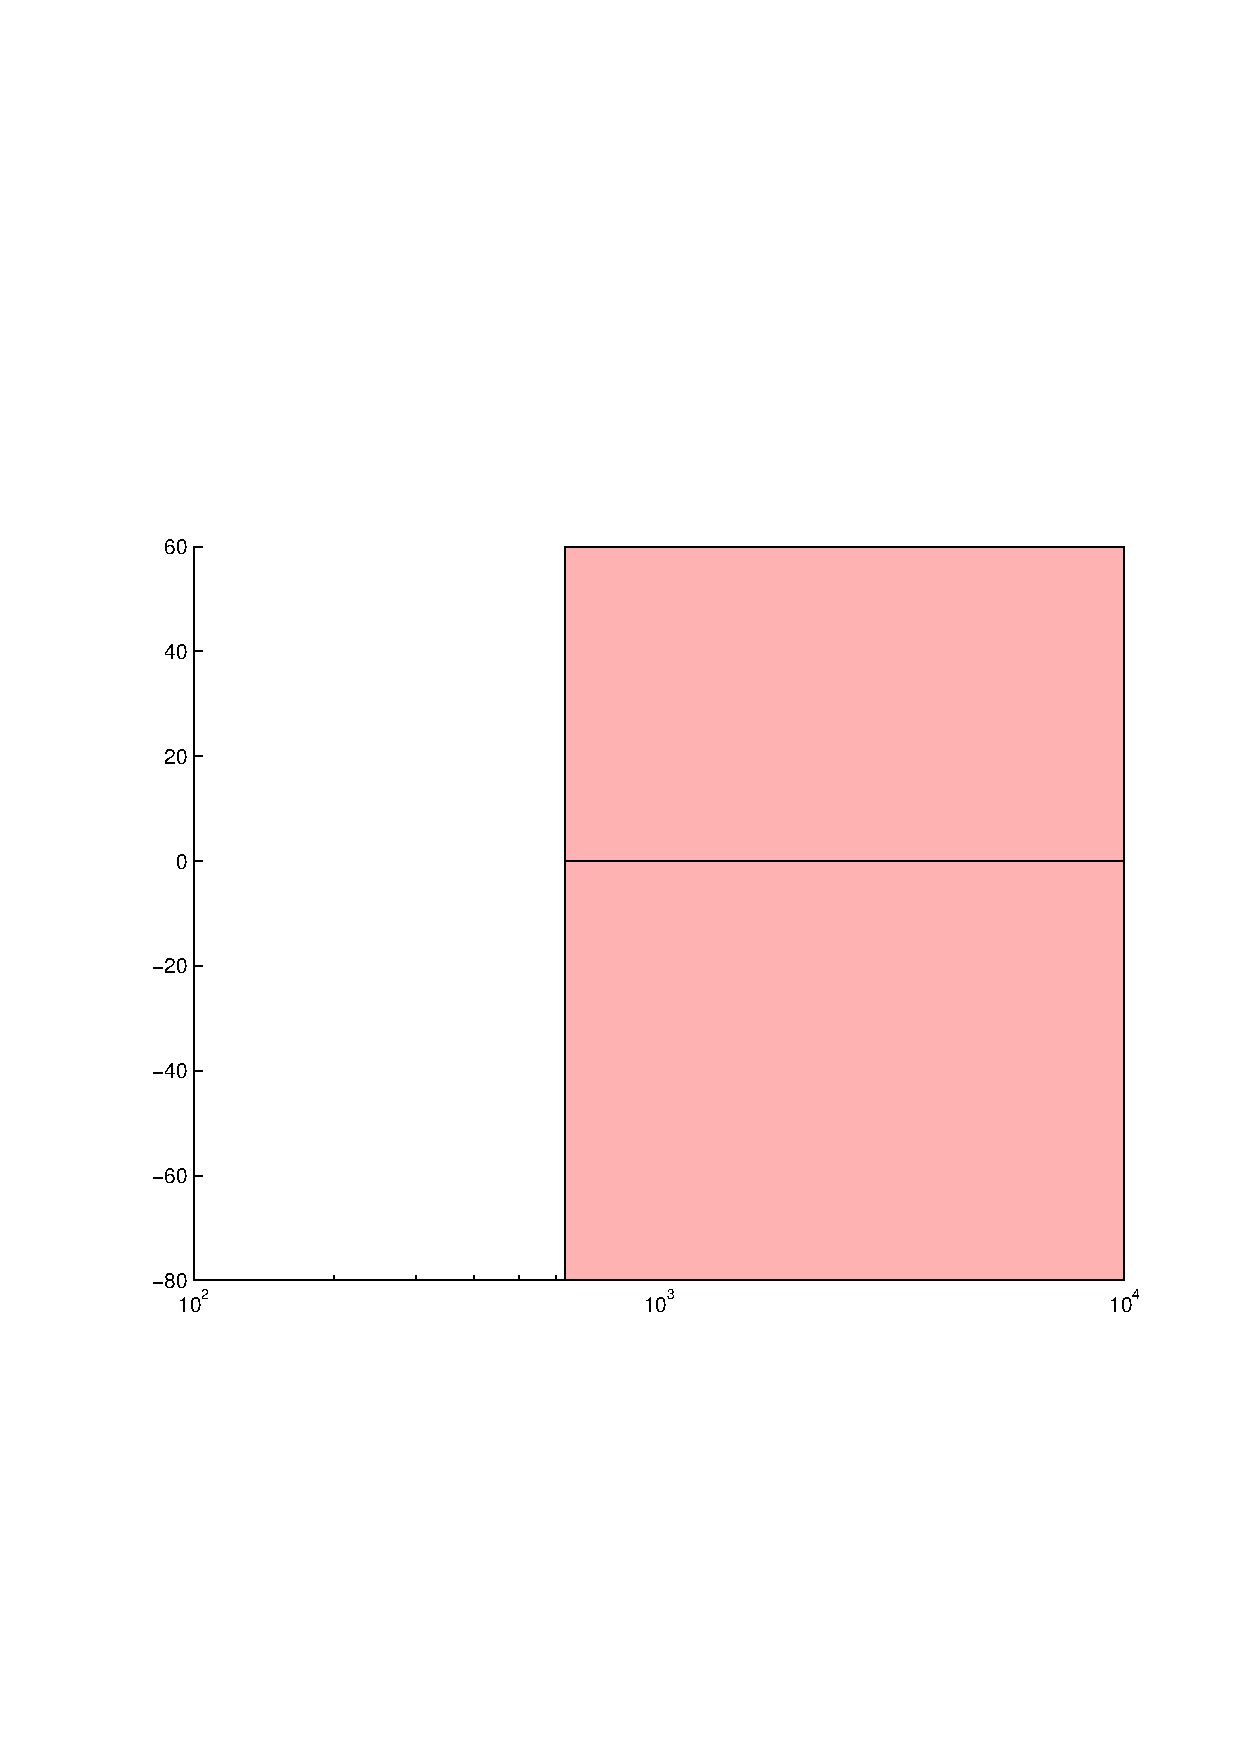
\includegraphics[scale=0.5]{gabarit4.pdf}
    \captionof{figure}{\textit{Diagramme illustrant le gabarit du rejet de bruit de mesure pour $S(p)$}}
    \label{fig10}
  \end{center}      

\paragraph{}
Arrivés à ce point, on pourra maintenant assembler tous nos gabarits et commencer à traiter les autres spécifications de notre cahier des charges. La figure suivante regroupe tous nos gabarits.\\

\begin{center}
    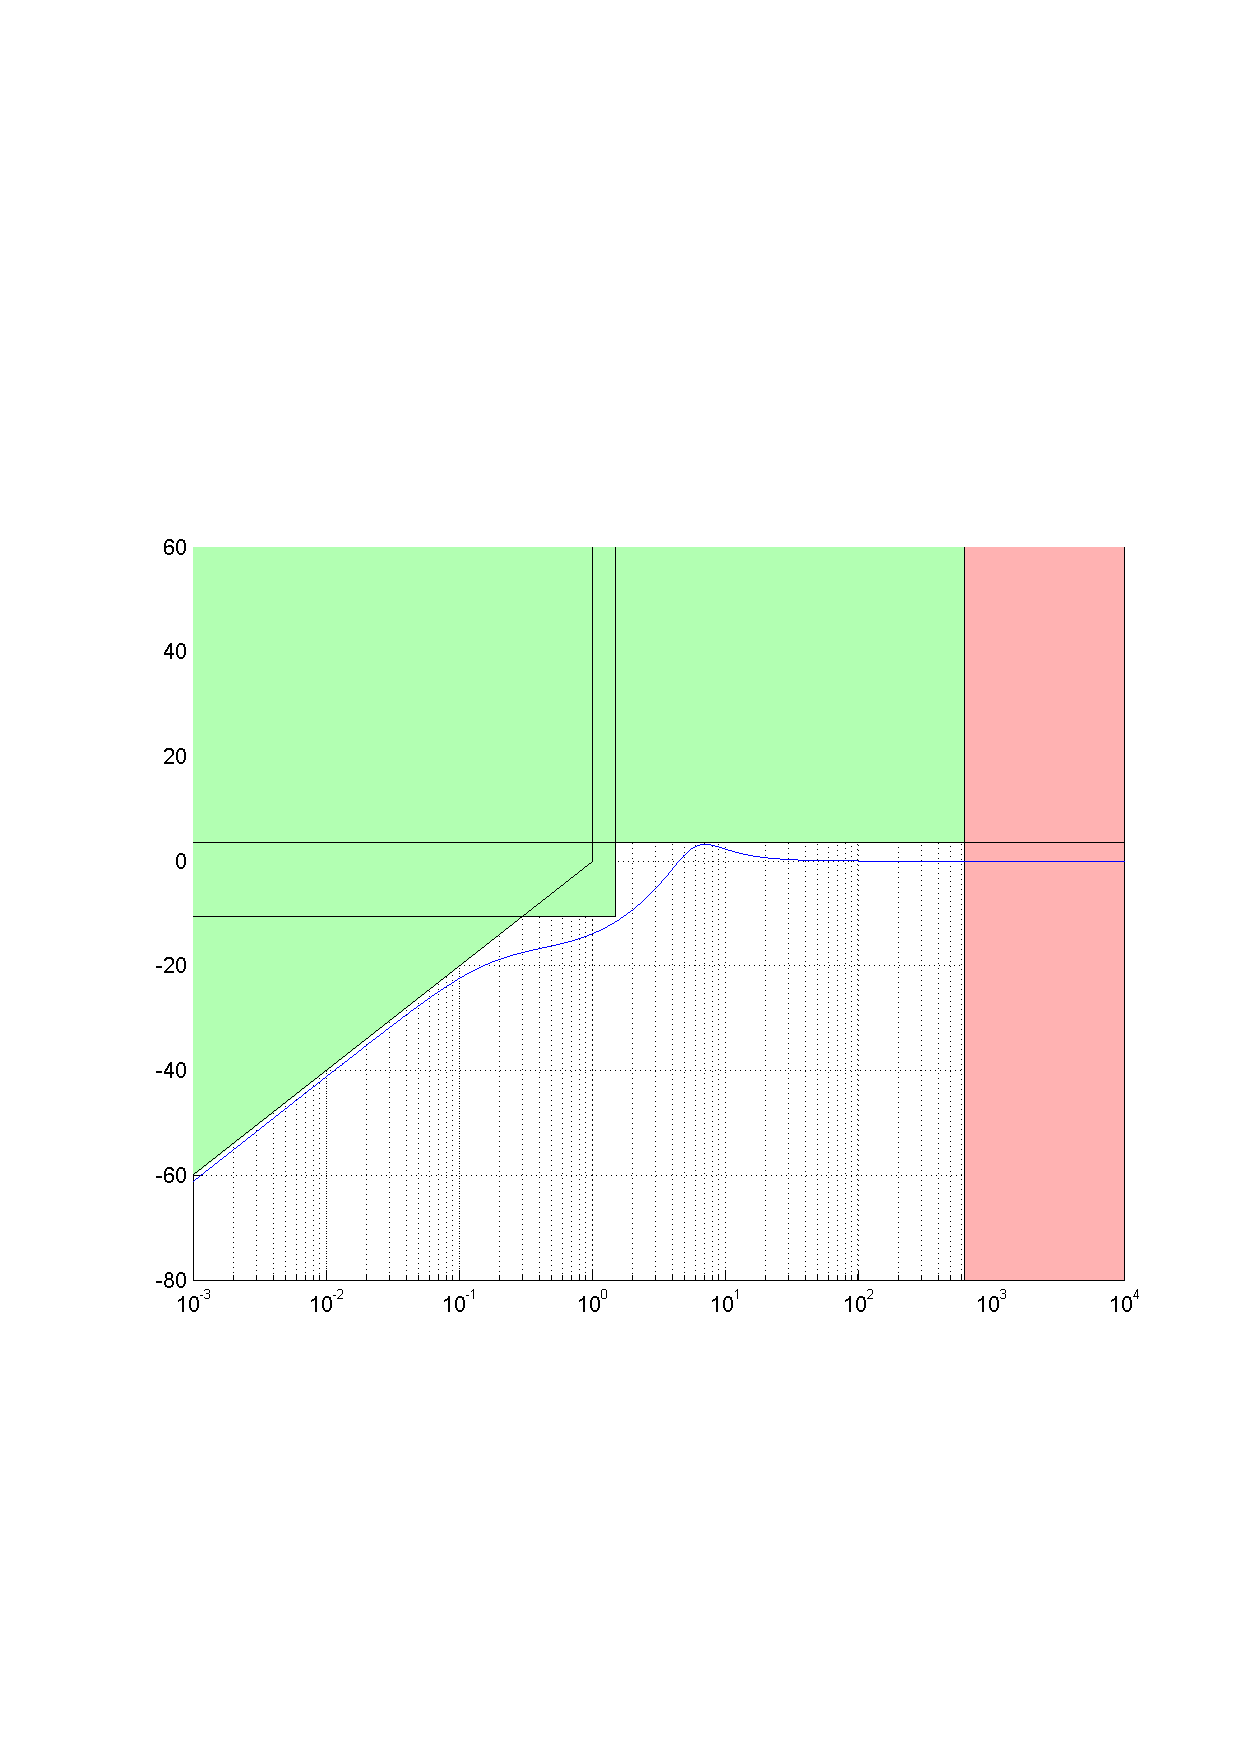
\includegraphics[scale=0.5]{touslesgabarits.pdf}
    \captionof{figure}{\textit{Diagramme illustrant tous les gabarits pour  $S(p)$}}
    \label{fig11}
  \end{center}

 \section{ Calcul de l'erreur de vitesse} 
 
 \paragraph{}
 On sait que: \hspace{1mm} $\xi_{v}=\underset{p\longrightarrow 0}{lim}\frac{S(p)}{p}$ \hspace{1mm} et que: \hspace{1mm}$S(p)=\frac{1}{1+G(jw)K(jw)}$\\[0.75mm]
 On trouve: $\xi_{v}=\underset{p\longrightarrow 0}{lim} \frac{\tau_{i}p^{4} + 7 \tau_{i} p^{3} + 12.75 \tau_{i}p^{2} + 6.75 \tau_{i}p }{4 \tau_{i}p^{5} + 7 \tau_{i}p^{4} + ( 16 k \tau_{i} + 12.75 \tau_{i} )p^{3} + ( 6.75 \tau_{i} + 16 k + 20 k \tau_{i} )p^{2} + 20 k p}$\\[0.75mm]
 L'équivalent basse fréquence de $\xi_{v}$ vaut alors: \hspace{1mm}$\frac{6.75 \tau_{i}}{20k} $ \\[0.75mm]
 Or: \hspace{1mm} $\xi_{v} \leqslant 1 \Rightarrow \frac{6.75 \tau_{i}}{20k} \leqslant 1$\\[0.75mm]
 \textbf{Conséquence:}\hspace{1mm} Maintenant qu'on a trouvé une relation entre $k$ \hspace{1mm} et $\tau_{i},$ \hspace{1mm} il nous est beaucoup plus facile de satisfaires nos gabarits.  
 
 \section{Tracé de Black - Nichols} 

 \begin{center}
     %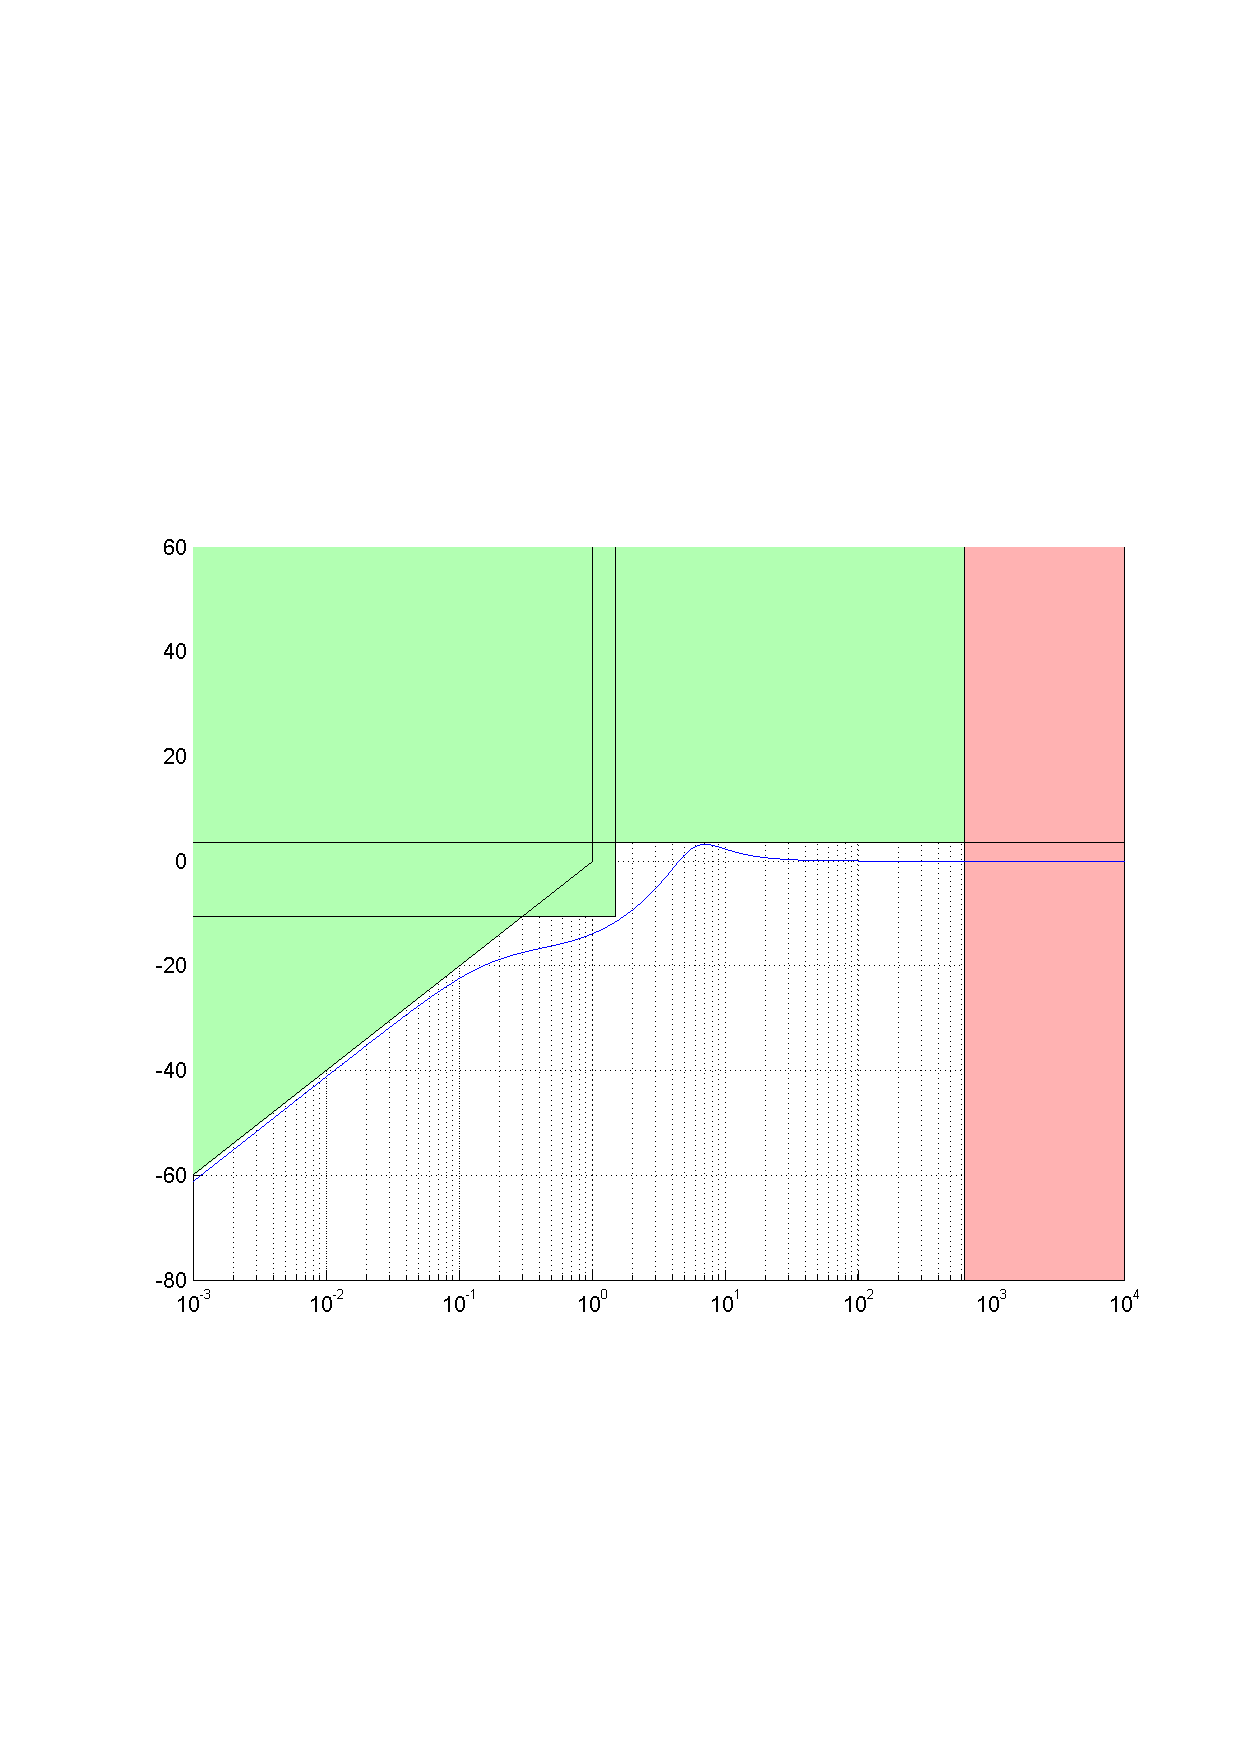
\includegraphics[scale=0.5]{touslesgabarits.pdf}
     \captionof{figure}{\textit{Tracé de Black de la boucle ouverte}}
     \label{fig12}
 \end{center}

  
 \section{Détermination de $k$ et de $\tau_{i}$, Niyquist}
    
  \subsection{Détermination de $k$ et de $\tau_{i}$}  
  
  \paragraph{}  
  En sachant qu'il existe une infinité de solutions,sur MATLAB on a commencé à faire varier la valeur du gain $k$\hspace{1mm}et de\hspace{1mm}$\tau_{i} $ afin de trouver une solution respectant notre  cahier des charges. Grâce à notre relation précédente on désormais que le rapport de $\tau_{i} $ et de  $k$ doit être inférieur  ou égale à la valeur: $\frac{20}{6.75} \simeq 2.963, $\hspace{1mm}ce qui nous a fait gagner beaucoup de temps.\\
  
 \begin{center}
     %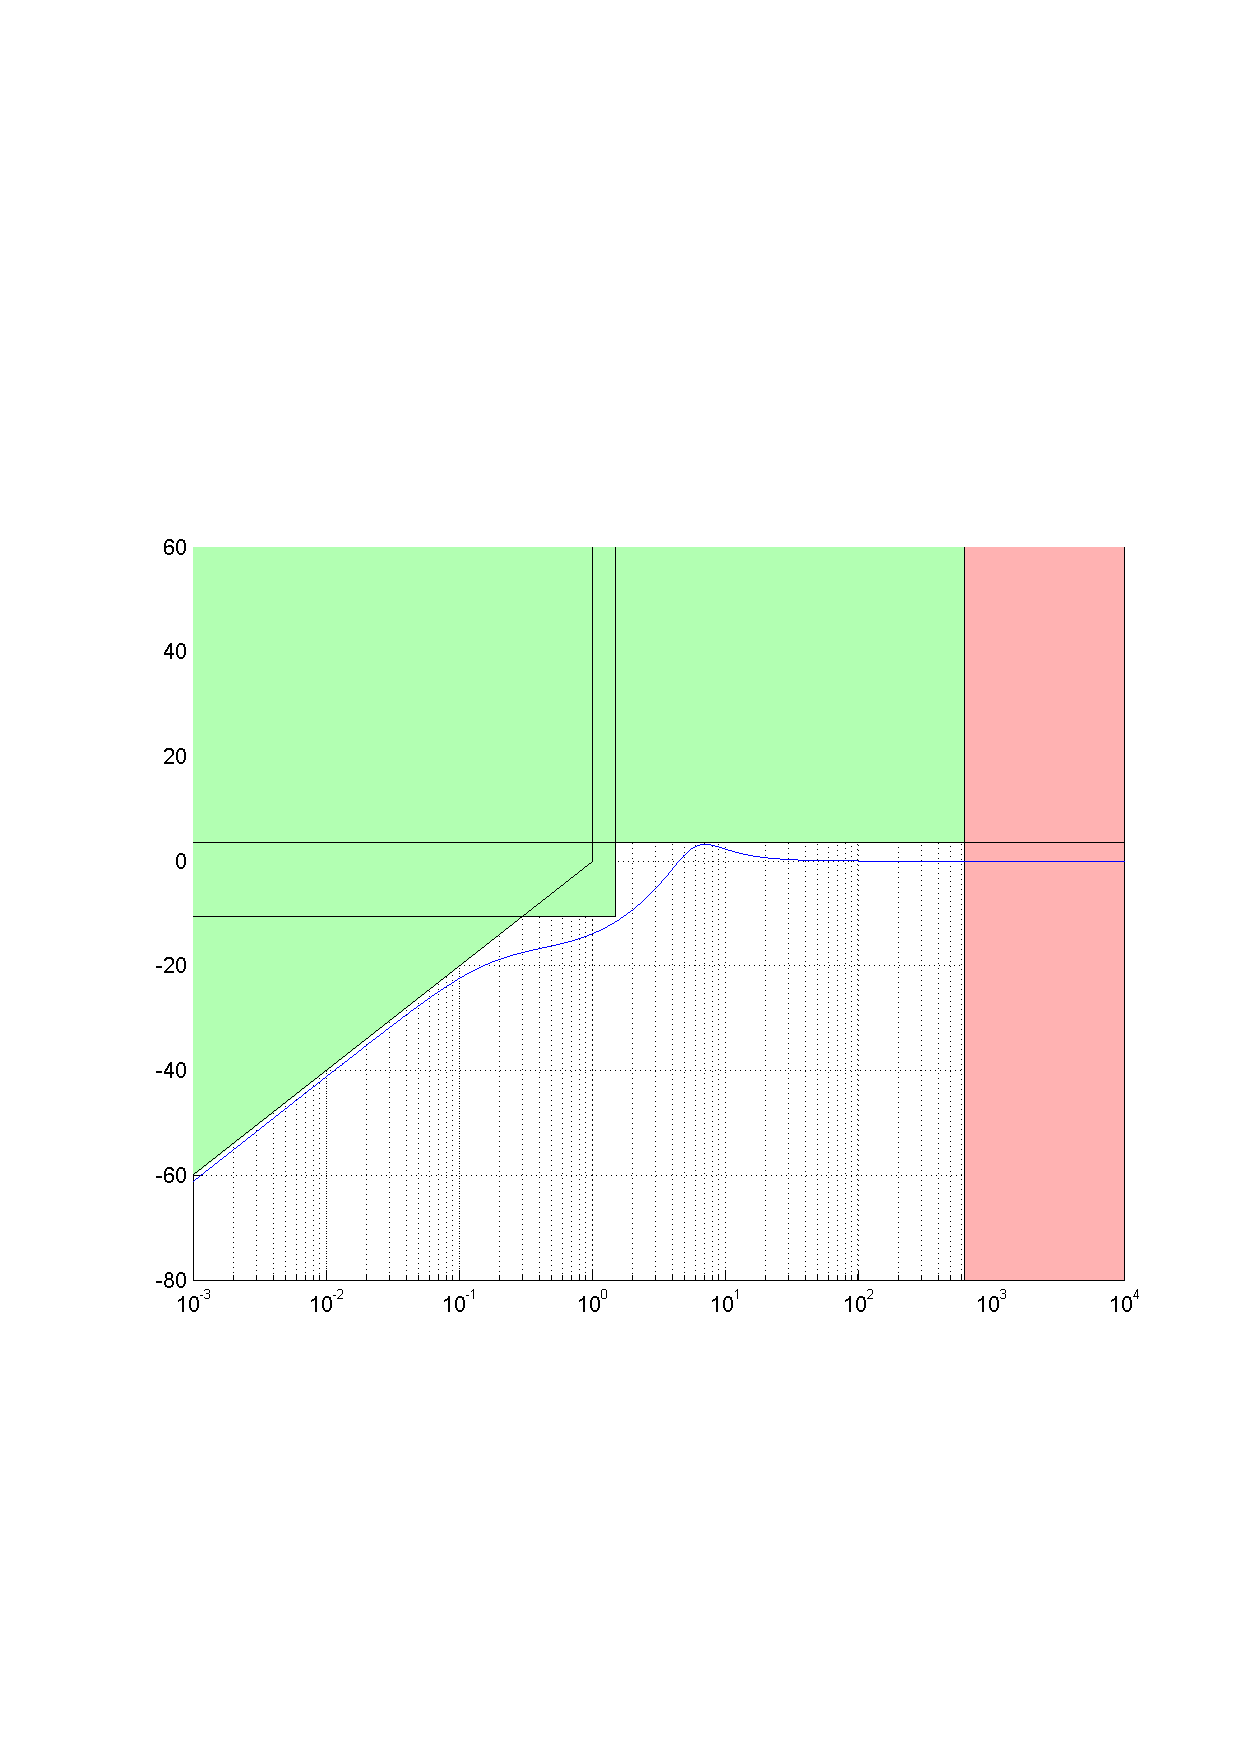
\includegraphics[scale=0.5]{touslesgabarits.pdf}
     \captionof{figure}{\textit{Tracés de $S(p)$ pour différentes valeurs de $k$ et de $ \tau_{i}$ }}
     \label{fig13}
 \end{center}
 
 \paragraph{}
 Arrivés à ce point, on pense que $k=0.335$ et $\tau_{i}=0.905505$ sont des solutions qui respectent le cahier des charges, nous allons garder ça pour plus tard. Vérifions maintenant que la courbe de $S(p)$ ne franchit pas les zones rouges c'est à dire le gabarit du rejet de bruit de mesure issu d'une condition nécéssaire. on sait que même si cette courbe franchie les zones vertes ça ne poserait pas problème car leurs gabarits sont issus de conditions suffisantes.\\
 
 
\begin{center}
     %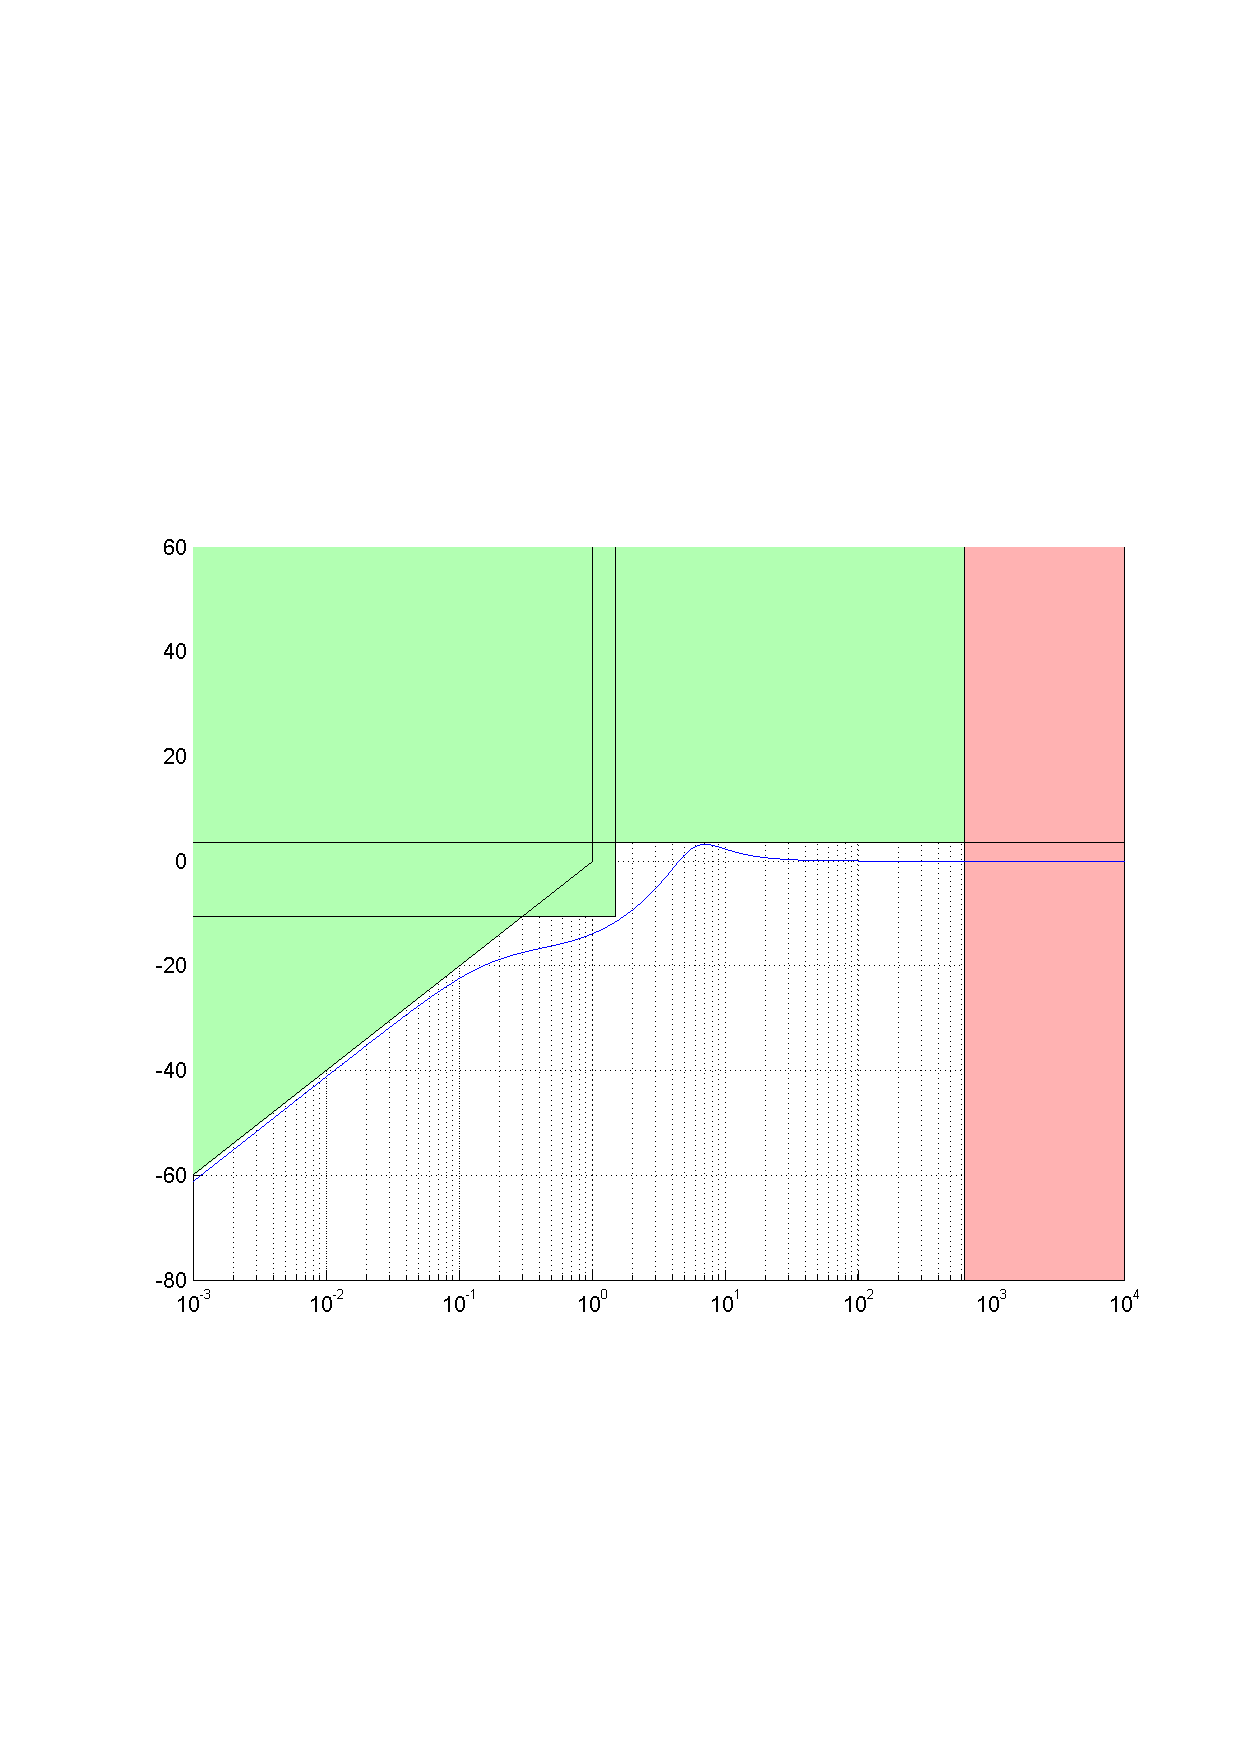
\includegraphics[scale=0.5]{touslesgabarits.pdf}
     \captionof{figure}{\textit{Tracé de $S(p)$ pour $k=0.335$ et $ \tau_{i}=0.905505$  }}
     \label{fig14}
 \end{center} 
 
 \begin{center}
     %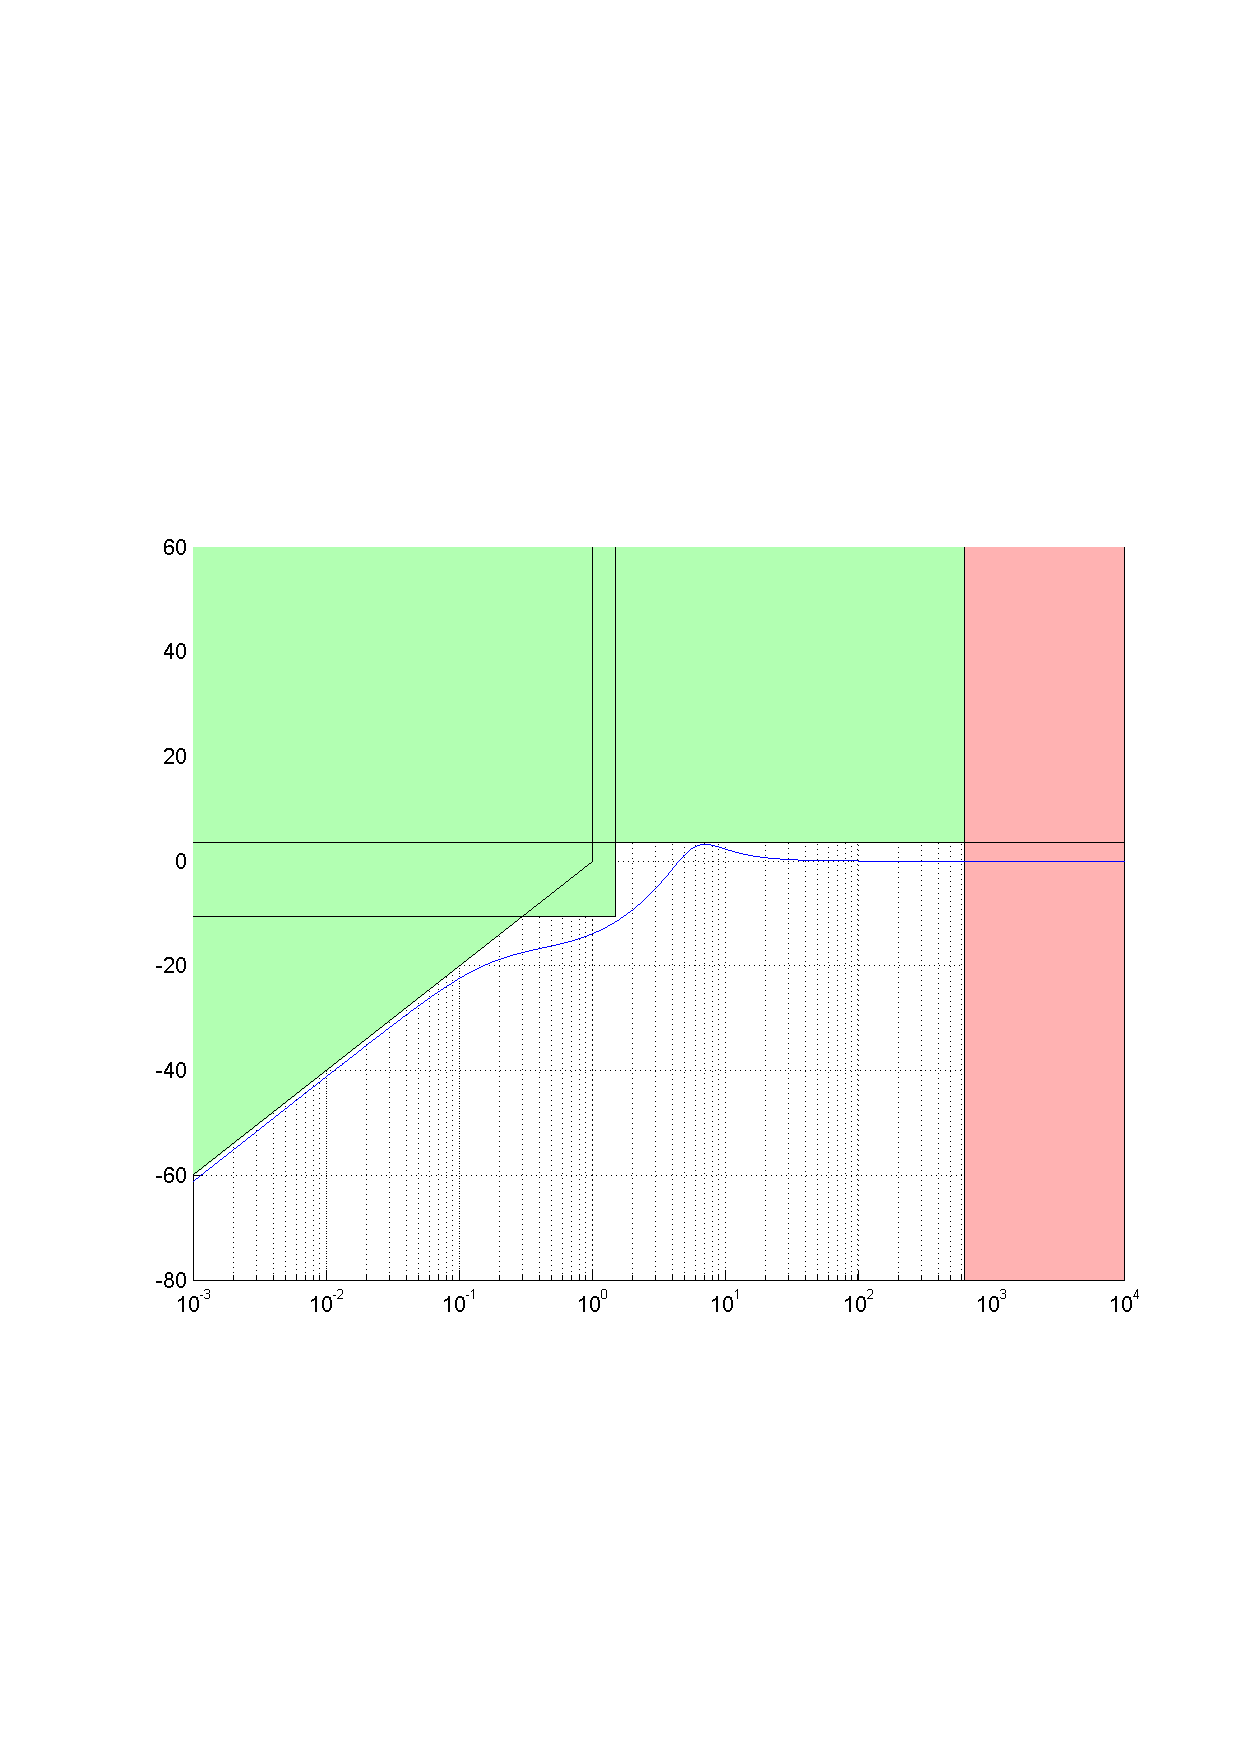
\includegraphics[scale=0.5]{touslesgabarits.pdf}
     \captionof{figure}{\textit{Vérification que $S(p)$ ne franchit pas les zones rouges }}
     \label{fig15}
 \end{center} 
 
  \subsection{Vérification de la stabilité par le critère de Nyquist}
   
   \paragraph{}
   Maintenant vérifions que la spécification de stabilité est vérifiée grâce au trac de Nyquist, nous rappelons que la courbe ne doit strictement pas dépasser la majorité de la partie gauche après la droite verticale au point -1.\\
   
   \begin{center}
     %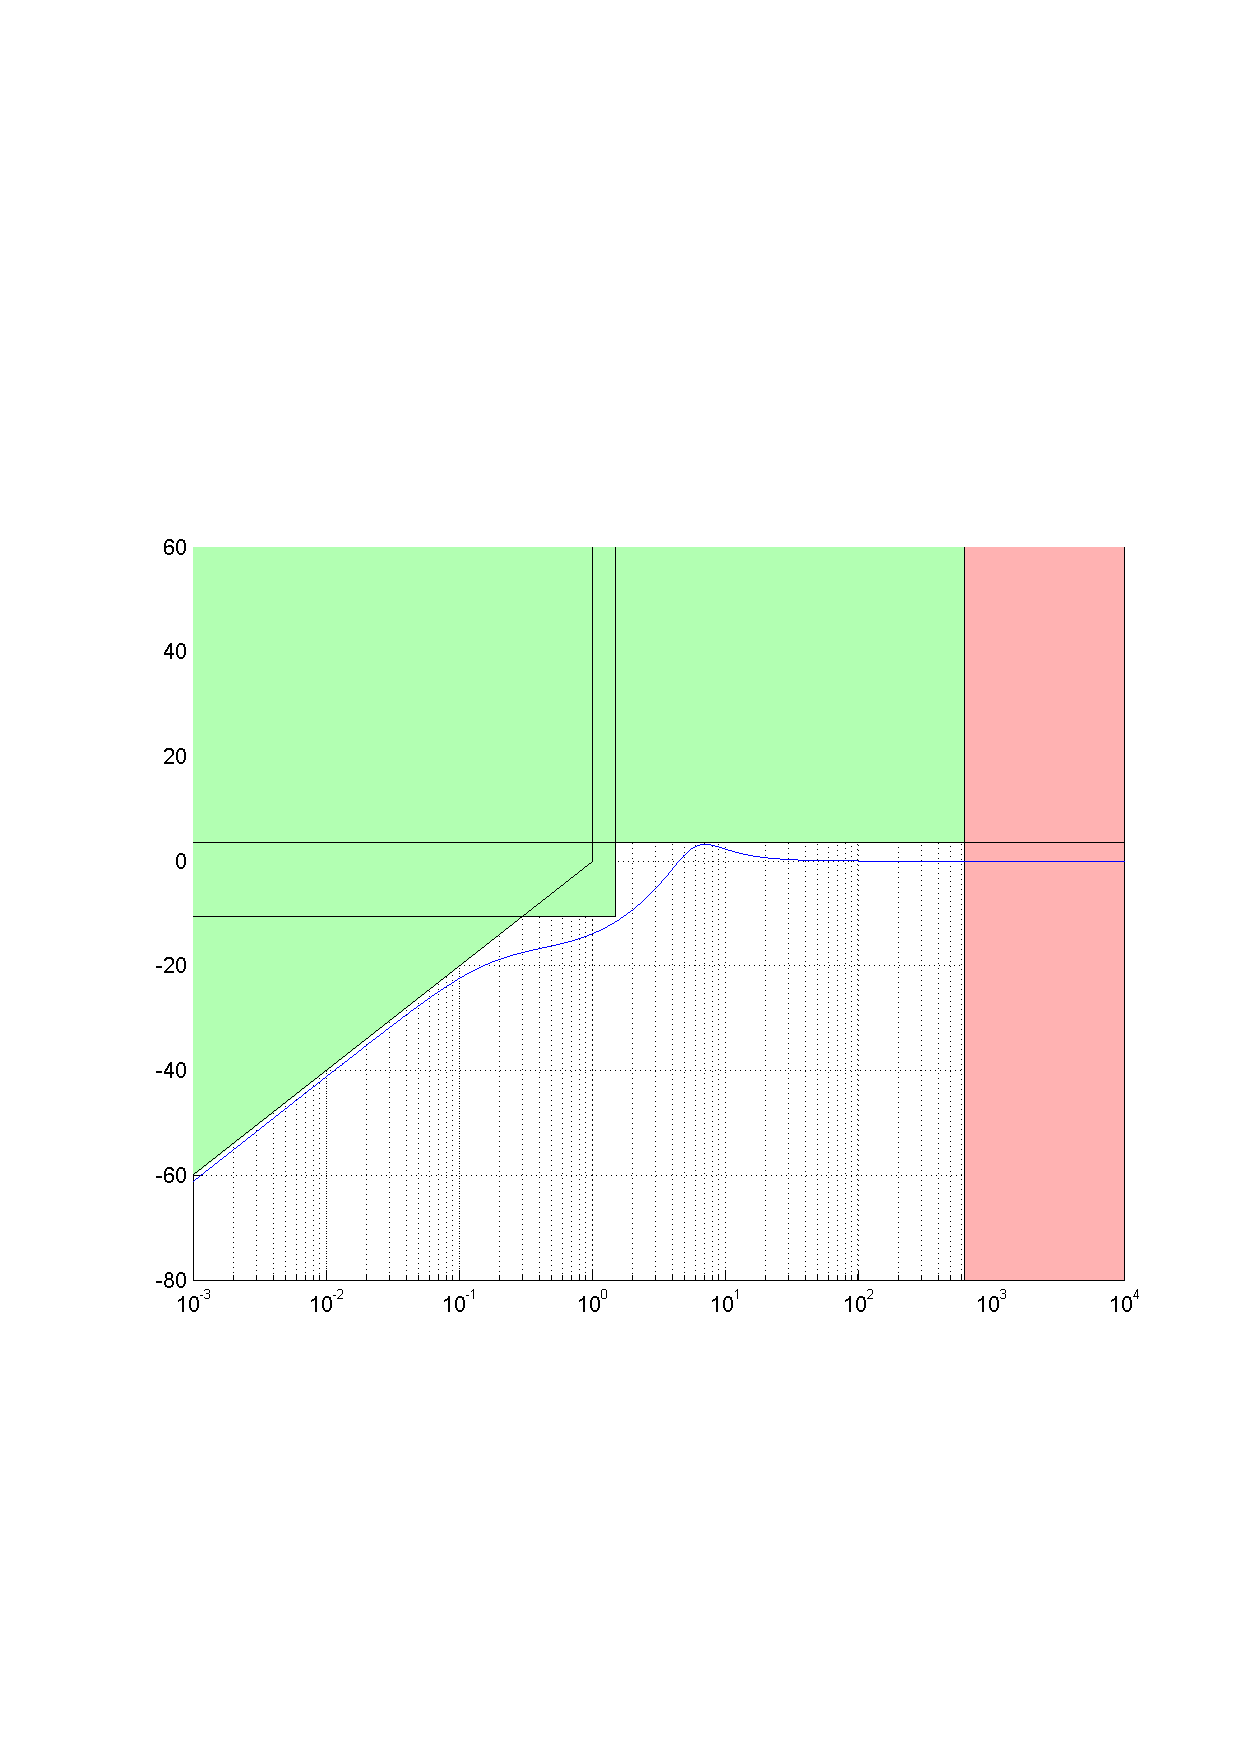
\includegraphics[scale=0.5]{touslesgabarits.pdf}
     \captionof{figure}{\textit{Tracé de Nyquist du $S(p)$ }}
     \label{fig16}
 \end{center}
 
  \section{ Tracés et calcul de la marge de module de $S(p)$\hspace{1mm} et de \hspace{1mm}$T(p)$}
  
   \subsection{ Tracés de $S(p)$\hspace{1mm} et de \hspace{1mm}$T(p)$}
   
   \begin{center}
     %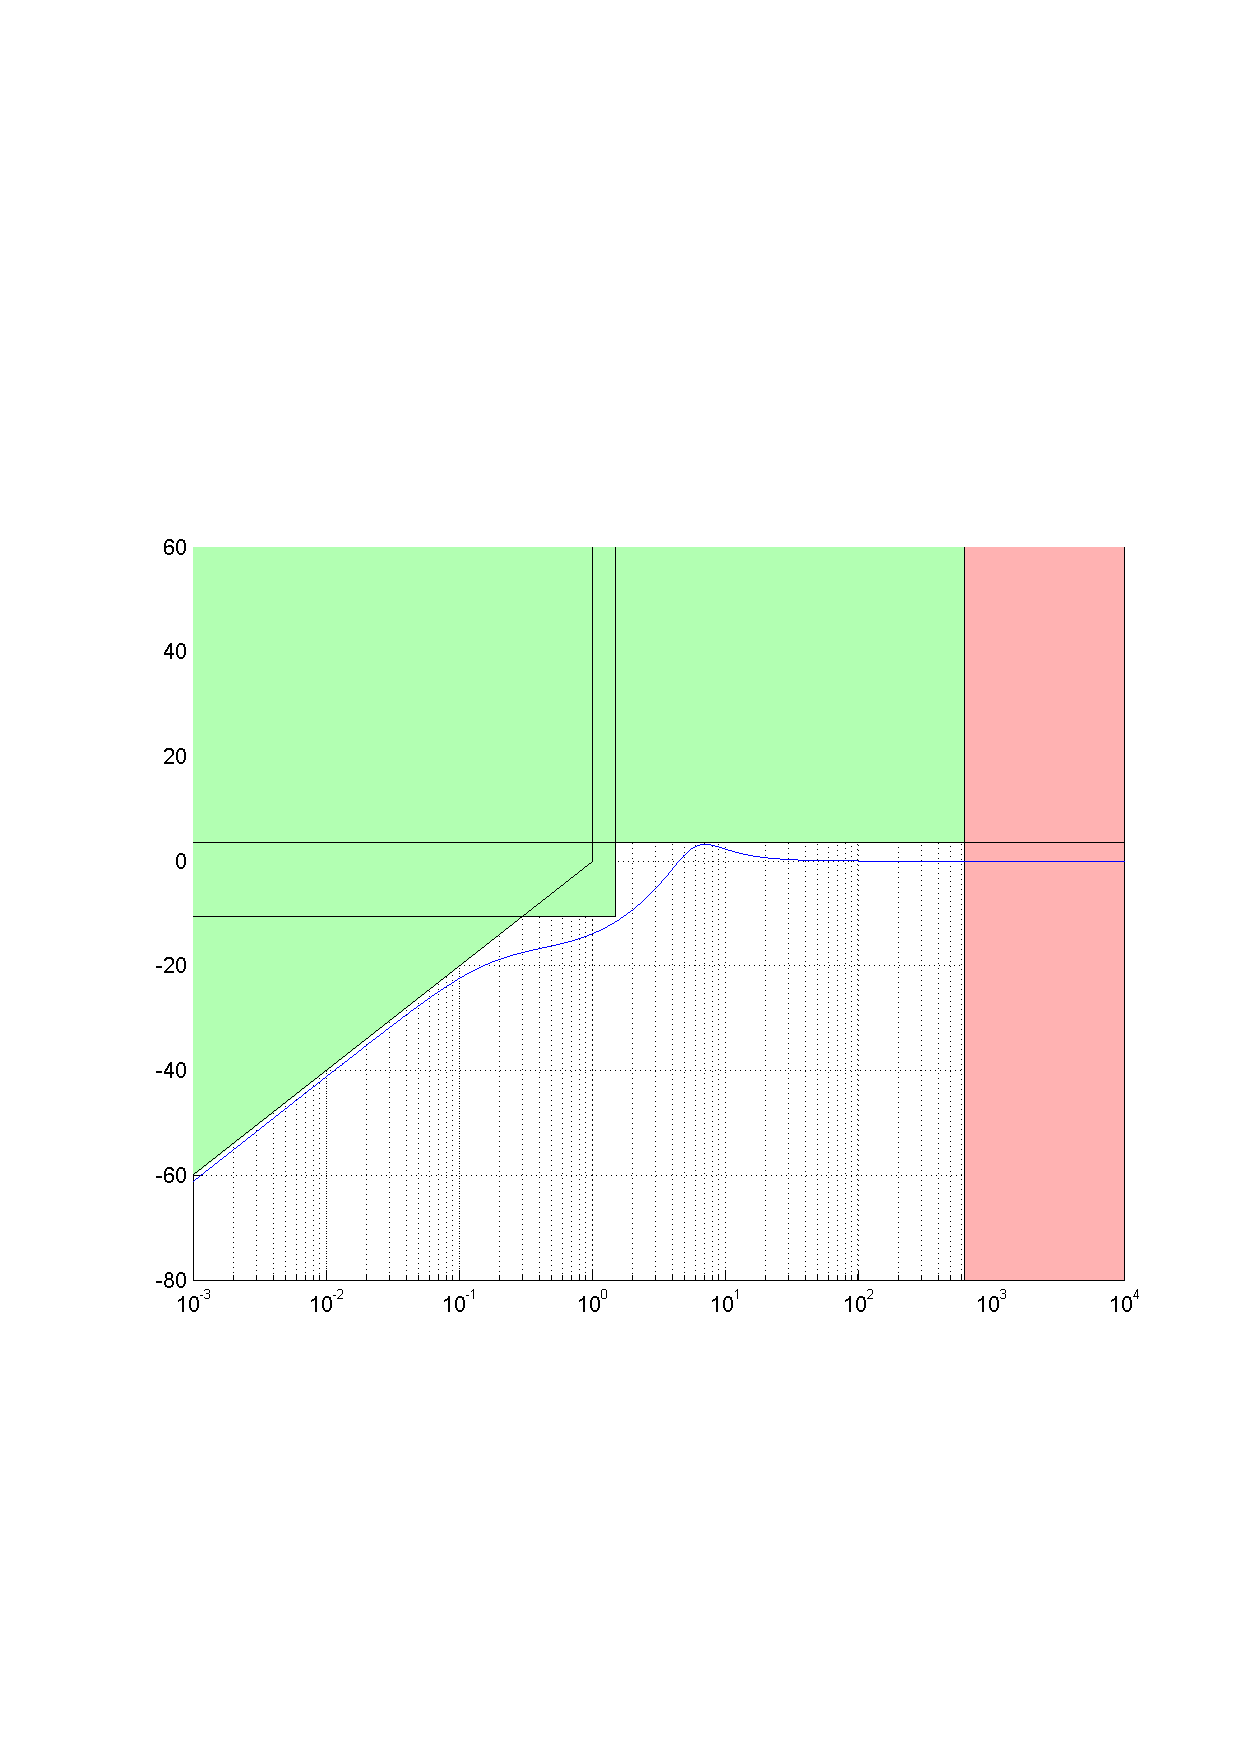
\includegraphics[scale=0.5]{touslesgabarits.pdf}
     \captionof{figure}{\textit{Feedback de $T(p)$}}
     \label{fig17}
 \end{center}
 

 %\paragraph{}
\textbf{Nota:} De cette courbe on obtient directement la valeur du temps de réponse qui vaut:\hspace{1mm} $2.92 s$\hspace{1mm} c'est à dire mois de\hspace{1mm} $3 s$, la spécification\hspace{1mm} $(d) $ \hspace{1mm}est respectée.   

% \paragraph{}
%\textbf{Nota:} De cette courbe on obtient directement la valeur de la pulsation à -3$dB$ c'est à dire la valeur de la pulsation de coupure $w_{c}$ qui vaut ici :\hspace{1mm} $1.34 rad.s^{-1}$ 
 
 \begin{center}
     %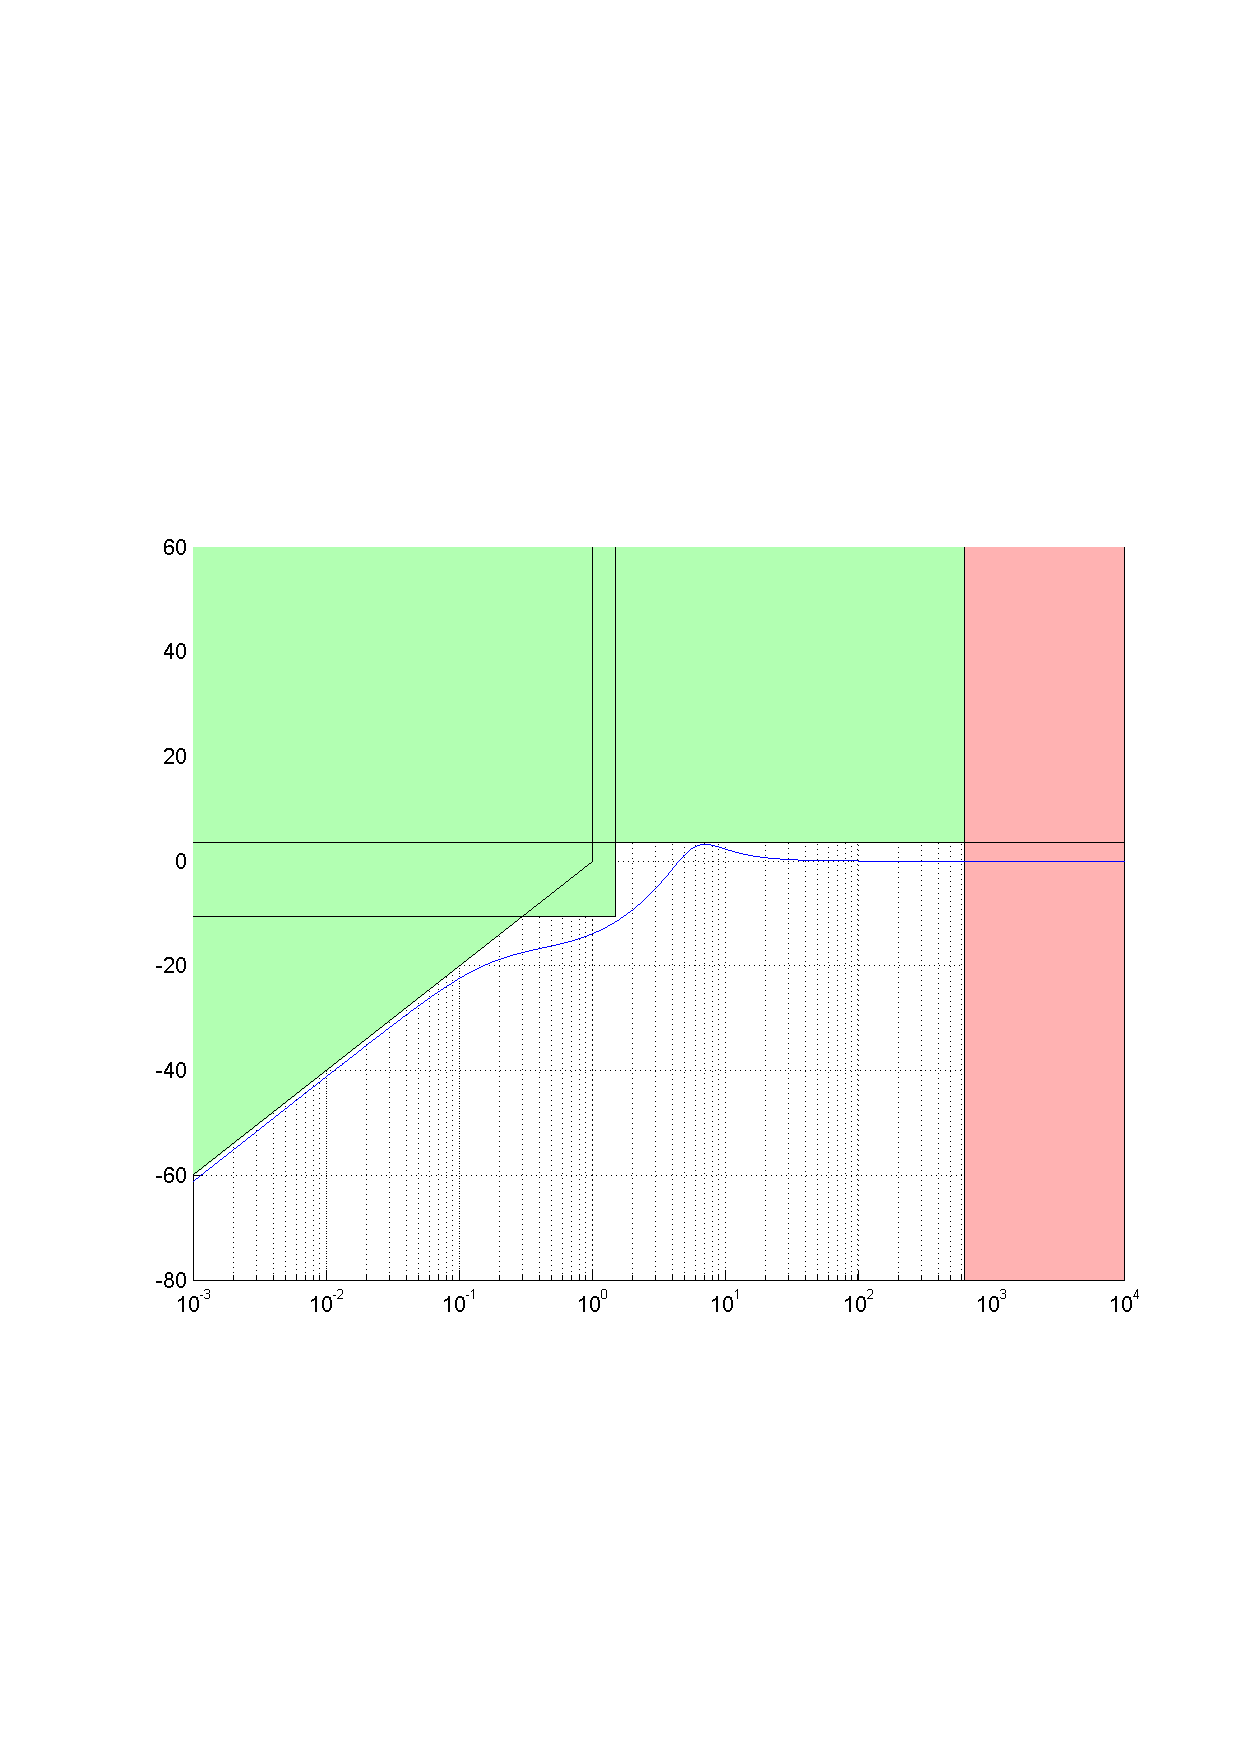
\includegraphics[scale=0.5]{touslesgabarits.pdf}
     \captionof{figure}{\textit{Feedback de $S(p)$}}
     \label{fig18}
 \end{center}
   
   \subsection{Calcul de la marge de module de $S(p)$\hspace{1mm} et de \hspace{1mm}$T(p)$} 
 
   \paragraph{}
   La marge de module de $S(p)$ vaut :
   
   \paragraph{}
   La marge de module de $T(p)$ vaut :
   
   \paragraph{}
\textbf{Conclusion:} %conclusion sur la robustesse du sys

  \section{ Tracé de la réponse indicielle et de la réponse à un échelon de perturbation}
  
  \subsection{Tracé de la réponse indicielle}
  
  \begin{center}
     %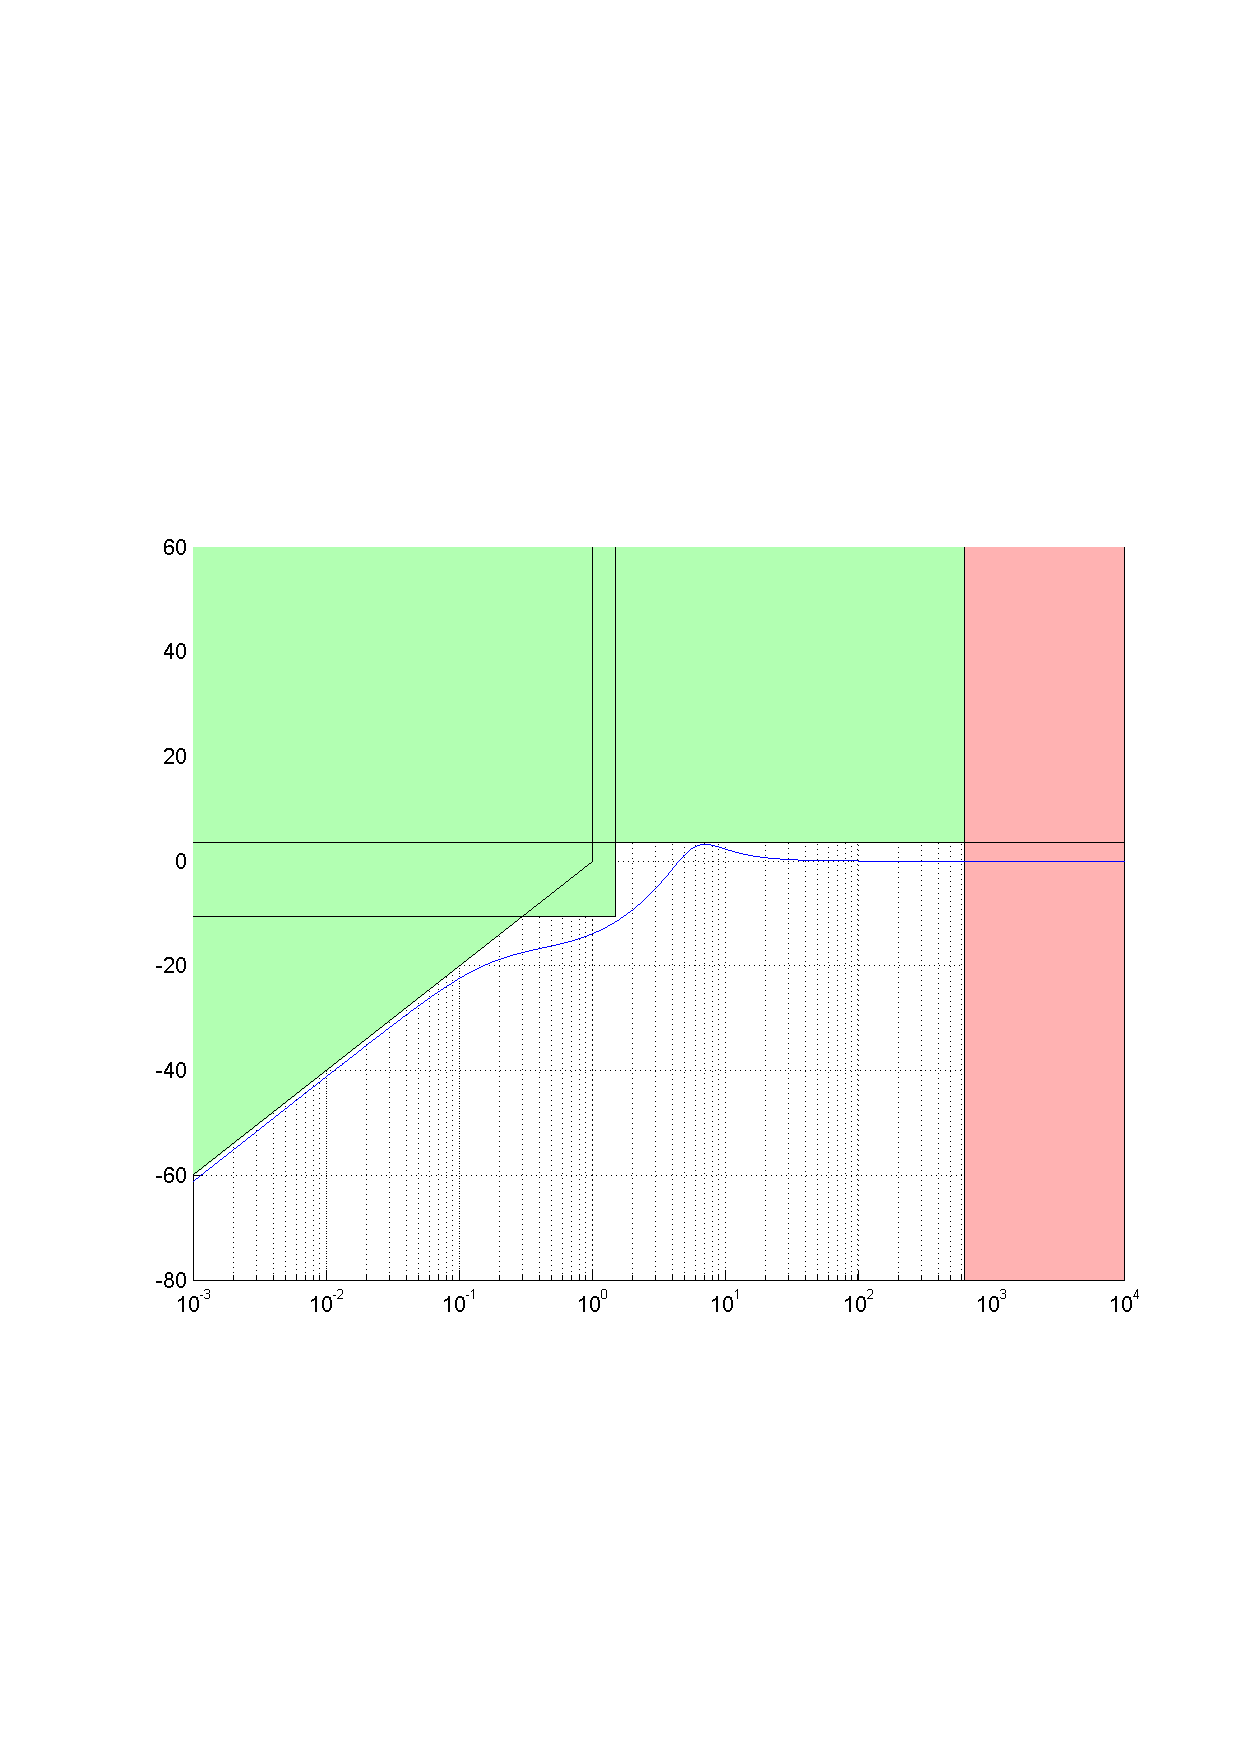
\includegraphics[scale=0.5]{touslesgabarits.pdf}
     \captionof{figure}{\textit{Reponse indicielle}}
     \label{fig18}
 \end{center}
  
  \subsection{Tracé de la réponse à un échelon de perturbation} 

\begin{center}
     %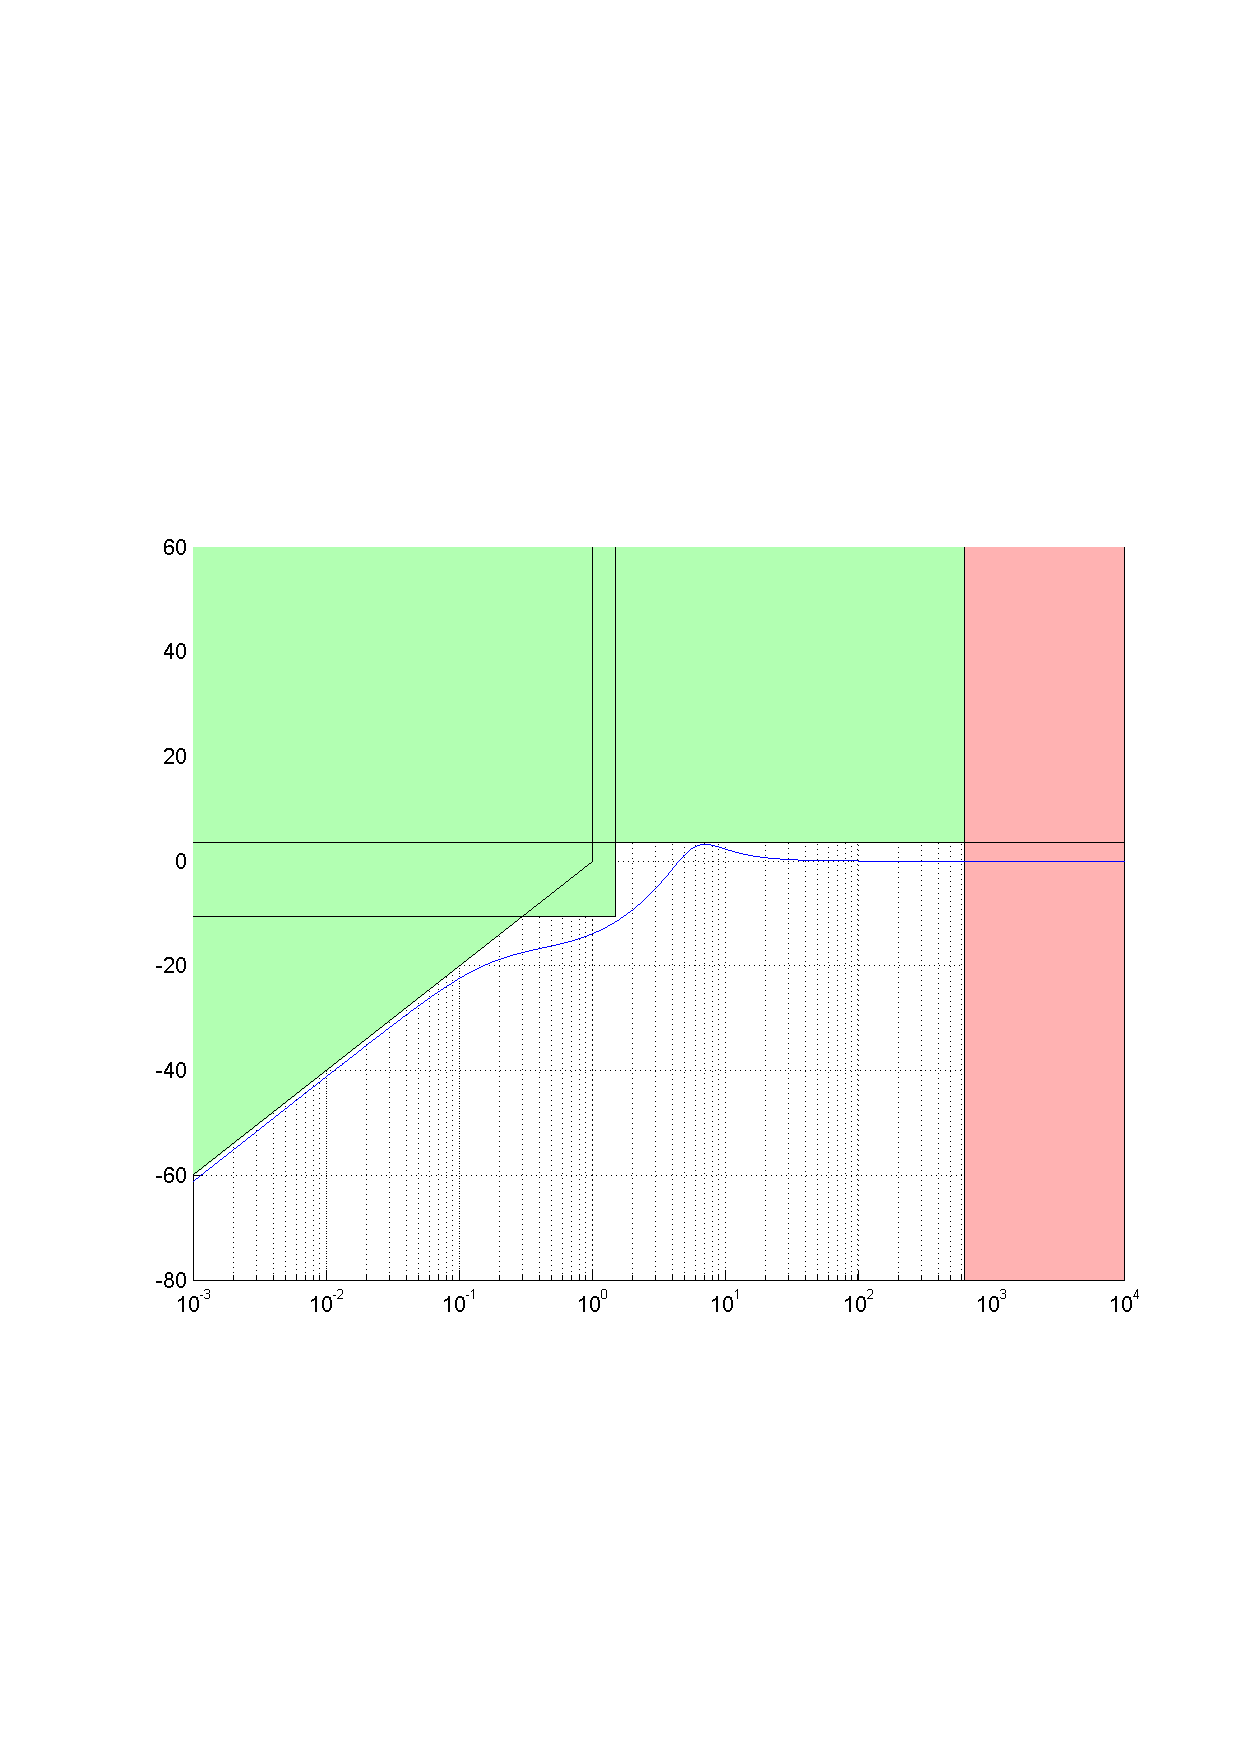
\includegraphics[scale=0.5]{touslesgabarits.pdf}
     \captionof{figure}{\textit{Reponse à un échelon}}
     \label{fig19}
 \end{center}
  
 \paragraph{}
 \textbf{Conclusion générale:} %sur le chapitre un et la 14eme question
 
\newpage
\paragraph{}

pour satisfaire cette condition ,il faut que $S(p)$ soit proche du zéro ,Donc il va falloir  que que $1+K(p)G(p)$ soit grand  pour que $S(p)$ converge vers zéro.
$ \forall_{\omega}, |W(p).S(p).G(p)|\leq \alpha \Rightarrow\ ||W(p).S(p).G(p)||_{\infty} \leq \alpha $ \\
On utilise le théorème de la valeur finale et on souhaite avoir un débit de fuite constante donc $W_{\mu}(p)= \frac{1}{P} $
On calcule l'erreur perturbation de commande $ \varepsilon_{c} $, on obtient $ G(0)S(0)=0 $ \\
Donc : $ \varepsilon_{c}=0 $

\paragraph{}
%question 3
On sait qu'une fonction du second ordre est de la forme : \\
$ \frac{1}{1+ \frac{2 \varepsilon }{ \omega_{n}} p + \frac{1}{ \omega_{n} ^ 2} p ^ 2} $ \\
On ajoute un Pole à $ L_{0}(p) $ \\

Donc : $ L_{0}(p)= \frac{1}{p} . \frac{1}{1+ \tau p} $ \\

La fonction de cosensibilité de ce système : \\
$ T(p) = \frac{L_{0}(p)}{1+ L_{0}(p)} $ \\
$ T(p) = \frac{1}{1 + p + \tau p^2}$ \\

On obtient donc aprés identification :

$ \frac{1}{\omega_{n}^2} = \tau $  \\

et \\
$ \frac{2 \varepsilon }{\omega_{n}} = 1 $ \\

Donc : \\

$ \varepsilon = 1  $ \\
On choisit un \varepsilon 1 pour ne pas avoir de dépassement et d’oscillation
$ \omega_{n} = 2 $ \\
$ \tau = 0.25 $ \\

On obtient donc : \\

$ L_{0}= \frac{1}{ p + 0.25 p^2 } $ \\

On obtient cette réponse fréquentielle dans le diagramme de black : \\

\begin{center}
     %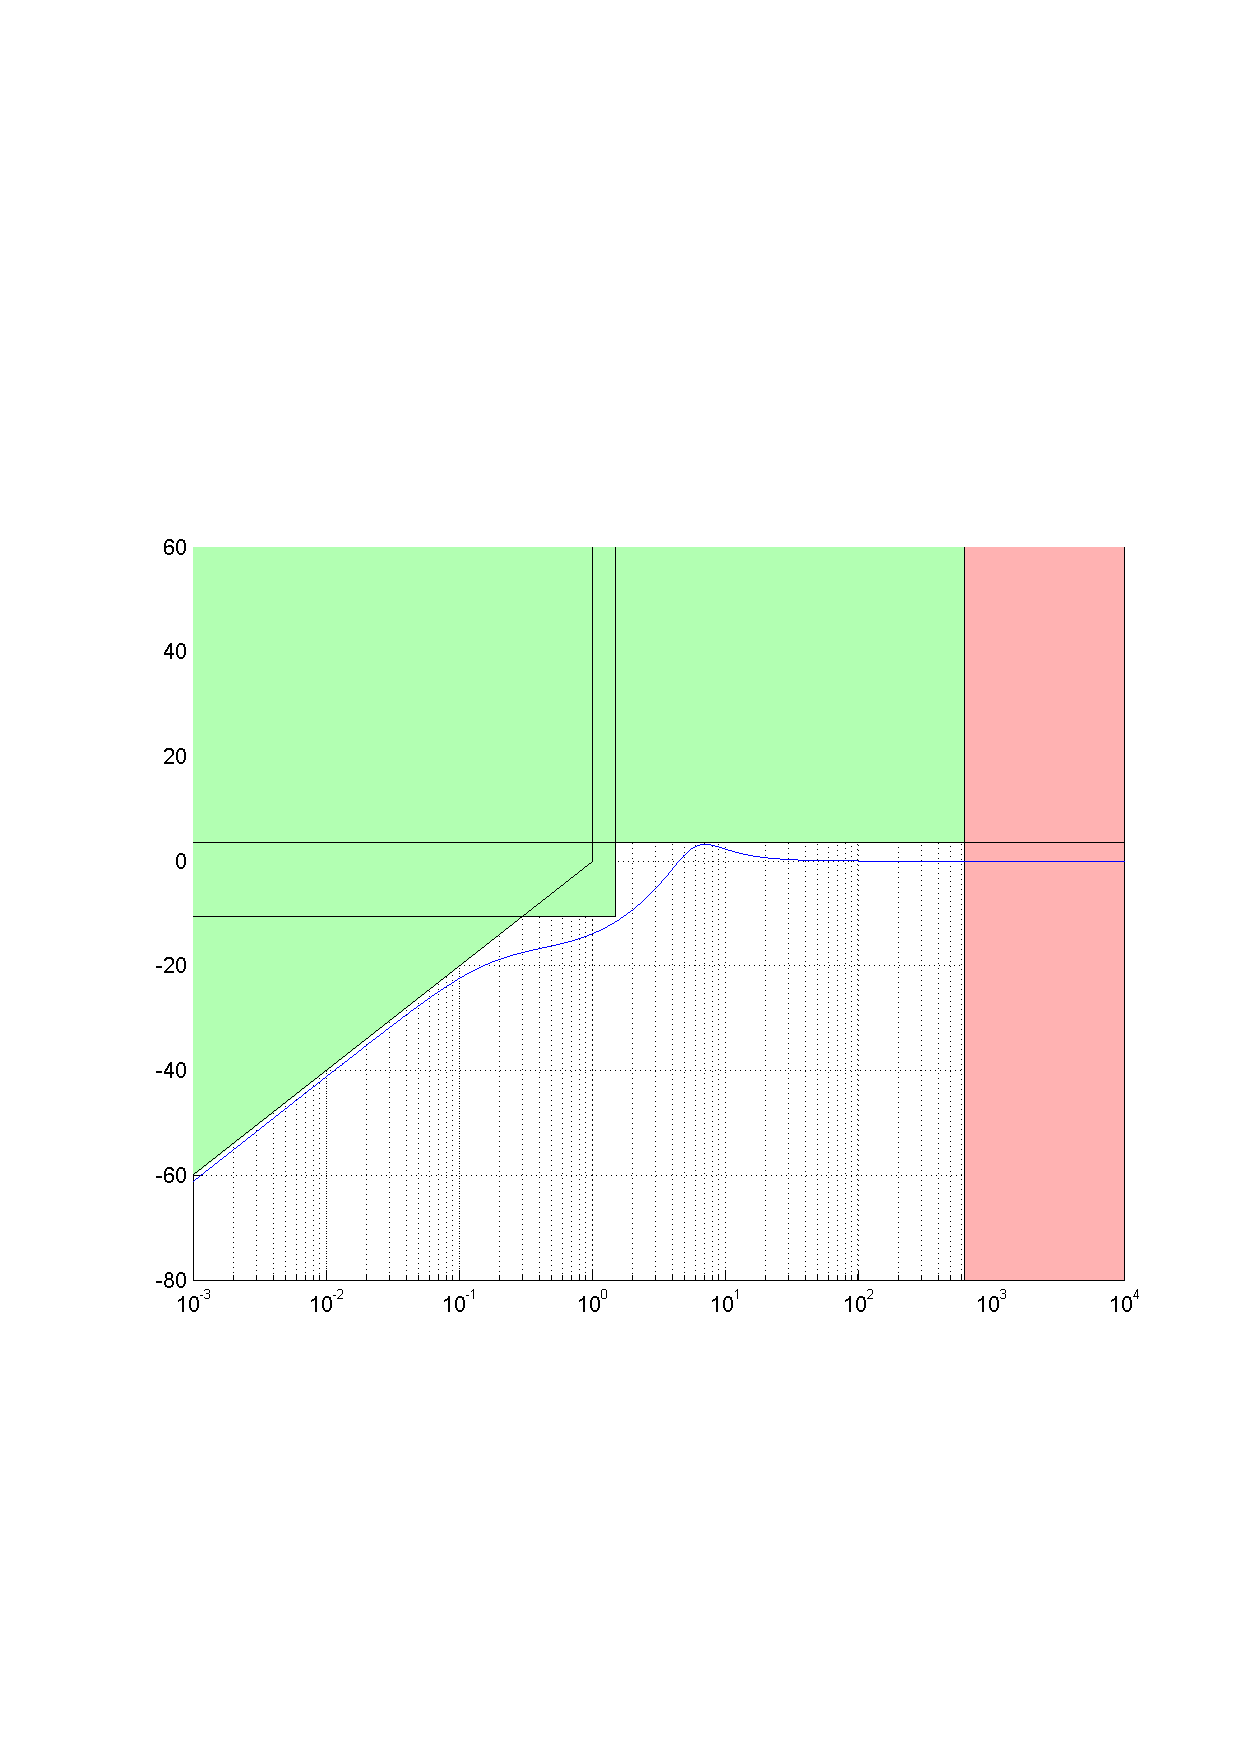
\includegraphics[scale=0.5]{touslesgabarits.pdf}
     \captionof{figure}{\textit{Réponse fréquentielle dans le diagramme de black  }}
     \label{fig}
 \end{center} 

%Titre : réponse fréquentielle dans le diagramme de black

\paragraph{}


On remarque que la  marge de phase est > à 45 degré et on notre courbre se trouve à droite du point de critique donc notre système est stable\\ 

%Question 4








%*********************** CONCLUSION **************
\chapter*{Conclusion}
 \addcontentsline{toc}{chapter}{Conclusion}
 
%*********************** Bibliographie ************ 
\bibliographystyle{alpha}
\bibliography{bibliographieperfoRobu}  

\chapter*{Annexe}
\begin{verbatim}
clear all
close all

% Trace d'un gabarit generique pour le TP

%% Parametrage :

w1 = 1; % Intersection de l'asymptote basse frequence avec l'axe des abscisses
n1 = 1; % Pente (*20dB/dec) de l'asymptote basse frequence

w2 = 1.37; % bande passante [0;w2] sur T / bande attenuee sur S
a2 = 1-(1/sqrt(2)); % facteur d'attenuation dans la bande attenuee de S

a3 = 100*exp(0.91*pi/(sqrt(1-0.91^2))); % norme Hinfinie maximale sur S//
%a3 = 100*exp(0.8*pi/(sqrt(1-0.8^2)));
w4 = 200*pi; % bande attenuee [w4;inf] sur T / canal de bande passante sur S //
a4_1 =0.999 ; % minimum d'amplitude dans le canal de bande passante sur S//
a4_2 = 1.001; % maximum d'amplitude dans le canal de bande passante sur S//

%% Trace du gabarit dans le diagramme de bode de S :

wlogmin = -3;
wlogmax = 4;
wmin = 10^wlogmin;
wmax = 10^wlogmax;
Gmin = -80;
Gmax = 60;
w = logspace(wlogmin,wlogmax,2000); % Echantillon de frequences en echelle log
figure(1);
ha = axes;
set(ha,'XScale','log');

hold on
h1=line([wmin w1 w1],[n1*20*log10(wmin/w1) 0 Gmax]);
h2=line([wmin w2 w2],[20*log10(a2) 20*log10(a2) Gmax]);
h3=line([wmin wmax],[20*log10(a3) 20*log10(a3)]);
h4_1=line([w4 w4 wmax],[Gmin 20*log10(a4_1) 20*log10(a4_1)]);
h4_2=line([w4 w4 wmax],[Gmax 20*log10(a4_2) 20*log10(a4_2)]);

%set([h1;h2;h3],'Color',[0 1 0]);
%set([h4_1;h4_2],'Color',[1 0 0]);

figure(2)
hab = axes;
set(hab,'XScale','log');

hold on
% h1b=patch([wmin w1 w1 wmin],[n1*20*log10(wmin/w1) 0 Gmax Gmax],[0.7 1 0.7]);
% print -dpdf gabarit1
h2b=patch([wmin w2 w2 wmin],[20*log10(a2) 20*log10(a2) Gmax Gmax],[0.7 1 0.7]);
%print -dpdf gabarit2
% h3b=patch([wmin wmax wmax wmin],[20*log10(a3) 20*log10(a3) Gmax Gmax],[0.7 1 0.7]);
% print -dpdf gabarit3
% h4_1b=patch([w4 w4 wmax wmax],[Gmin 20*log10(a4_1) 20*log10(a4_1) Gmin],[1 0.7 0.7]);
% h4_2b=patch([w4 w4 wmax wmax],[Gmax 20*log10(a4_2) 20*log10(a4_2) Gmax],[1 0.7 0.7]);
% print -dpdf gabarit4
grid on
%set([h1b;h2b;h3b],'FaceAlpha',0.2);
%set([h4_1b;h4_2b],'FaceAlpha',0.2);

%% Trace initial du diagramme de Bode de S
%%kk=0.335;
kk=0.3713;
%max 2.3
%a=20/6.75 = 2.963 qu'il ne faut absolument pas depasser

a=2.703;


%%tt=a*kk;
tt=1.1;
ng=[16 20];
dg=[1 7 12.75 6.75];
nk=[kk*tt kk];
dk=[tt 0];
%%%Boucle ouverte
zs=tf(ng,dg)*tf(nk,dk);
%% Sensibilite
ss=1/(1+zs);
%% T 
t=zs*ss;  % cosensibilite
%%S = tf([1 2 0],[1 1 5]);
%%GS = 20*log10(squeeze(abs(freqresp(S,w))));
GS = 20*log10(squeeze(abs(freqresp(ss,w))));
hBodeS = plot(w,GS,'b-');
grid on

%print -djpeg touslesgabarits

%% Iteration du trace

%%S = tf([1 2 0],[1 1 5]);
%%GS = 20*log10(squeeze(abs(freqresp(S,w))));
%GS = 20*log10(squeeze(abs(freqresp(ss,w))));
set(hBodeS,'YData',GS);



%GSS = 20*log10(squeeze(abs(freqresp(t,w))));

%%Bode de T pour trouver wc pulsation de coupure
figure(3)
bodemag (t);
grid on
%hBodeS = plot(w,GSS,'b-');



%% Feedback de T    question 12

feed= feedback(t,1);
%feed2= feedback(tf(kk,[1 0]),1);
figure(4)
step(feed);
%hold on 
%step(feed2);
grid on

%%Feedback de S question 12
feed3= feedback(ss,1);
figure (8)
step(feed3);

%% Bode asymptotique question 2
bod=tf(nk,dk);
figure (5)
bode(bod)
grid on

%% Black boucle ouverte 
figure (6)
nichols(zs);

%% Nyquist de S pour dire que notre systeme est stable loin du popint -1 question 11
figure (7)
nyquist(ss);


\end{verbatim}

\end{document}

